\documentclass[t]{beamer}

% Load general definitions
% Preamble file - general definitions, package loading, etc.

%=================================
% Load packages
\usepackage{amssymb,amsmath}
\usepackage{graphicx}
\usepackage{url}
\usepackage{tikz}
\usetikzlibrary{mindmap,trees,arrows}
\usepackage{fancyvrb}
\usepackage[portuguese]{babel} 
\usepackage[utf8]{inputenc}
\usepackage{subfigure}
\usepackage{times}
\usepackage[T1]{fontenc}
\usepackage{cancel}
\usepackage{color}
\usepackage{listings}
\usepackage[document]{ragged2e}
\usepackage{physics}
\usepackage{amsmath}
\usepackage{tikz}
\usepackage{mathdots}
\usepackage{yhmath}
\usepackage{cancel}
\usepackage{color}
\usepackage{siunitx}
\usepackage{array}
\usepackage{multirow}
\usepackage{amssymb}
\usepackage{gensymb}
\usepackage{tabularx}
\usepackage{extarrows}
\usepackage{booktabs}
\usetikzlibrary{fadings}
\usetikzlibrary{patterns}
\usetikzlibrary{shadows.blur}
\usetikzlibrary{shapes}

%=================================
% Set mode
\mode<presentation>
{
	\usetheme{Madrid}
	\usecolortheme{structure}
	\useoutertheme{infolines}
	\setbeamercovered{invisible}
}

% Get rid of nav bar
\beamertemplatenavigationsymbolsempty

% Insert frame number at bottom of the page.
\usefoottemplate{\hfil\tiny{\color{black!90}\insertframenumber}} 

%=================================
% Define new commands

\newcommand\Real{{\mathbb{R}}}
%\newcommand{\vi}{\vspace{0.6\baselineskip}}
%\newcommand{\goodgap}{\hspace{\subfigtopskip}\hspace{\subfigbottomskip}}


% Equation environments
\newcommand{\beq}{\begin{equation}}
\newcommand{\eq}{\end{equation}}
\newcommand{\beqs}{\begin{equation*}}
\newcommand{\eqs}{\end{equation*}}
\newcommand{\beqn}{\begin{eqnarray}}
\newcommand{\eqn}{\end{eqnarray}}
% Bold variables
\newcommand{\mbf}[1]{\ensuremath{\mathbf{#1}}}
% Itemization
\newcommand{\bitem}{\begin{itemize}}
\newcommand{\eitem}{\end{itemize}}
\newcommand{\spitem}{\vskip 1em\item}
\newcommand{\bitems}{\begin{itemize}\item}
\newcommand{\benums}{\begin{enumerate}\item}
\newcommand{\eenum}{\end{enumerate}}
% color blocks
\newenvironment{colorblock}[2]{%
\setbeamercolor{block title}{#2}
\begin{block}{#1}}{\end{block}}
% Vertical spacing
\newcommand{\vone}{\vskip 1em}
\newcommand{\vhalf}{\vskip .5em}
% Frame environments
\newenvironment{ftst}[3][t]{%
\begin{frame}{environment=ftst,#1}
\frametitle{#2}
\framesubtitle{#3}}{\end{frame}}
\newenvironment{ftstf}[2]{
\begin{frame}[fragile,environment=ftstf]
\frametitle{#1}
\framesubtitle{#2}}{\end{frame}}
% colors
\definecolor{MyGray}{rgb}{0.5,0.5,0.5}
\definecolor{MyDBGray}{rgb}{0.1,0.1,0.4}
\definecolor{darkgreen}{rgb}{0,0.4,0}
\definecolor{black}{rgb}{0,0,0}
\def\defn#1{{\color{red} #1}}
% Footnote
\renewcommand{\thefootnote}{\alph{footnote}}
% Relaxed footnotes
\newcommand{\lfr}[1]{\let\thefootnote\relax\footnote{\tiny #1}}
% Verbatim environment - using FANCYVRB package
\DefineVerbatimEnvironment%
{rcode}{Verbatim}
{fontsize=\scriptsize}
% Verbatim environment - using LISTINGS package
%\lstnewenvironment{rcode} {\lstset{	language = R,
%									basicstyle = \scriptsize\ttfamily,
%									showspaces = false,
%									showstringspaces = false,
%									showtabs = false,
%									keywordstyle = \color{black}\bfseries,
%									commentstyle = \color{darkgreen},
%									numbers = none,
%									otherkeywords={	<-,
%													ggplot,
%													geom_boxplot,
%													facet_grid,
%													shapiro.test,
%													fligner.test,
%													glht,
%													with},
%									deletekeywords={data,
%													model,
%													residuals,
%													c,
%													axis,
%													default,
%													labels,
%													qq.text}}}%
%{}

% Specific definitions
\title[]{Banco de dados II}
\subtitle[]{O Modelo Entidade-Relacionamento (MER)}
\author[]{Patrícia Lucas\\{\footnotesize }}
\institute{Bacharelado em Sistemas de Informação \\ IFNMG  - Campus Salinas}
\date{\scriptsize Salinas\\Julho 2021}

\begin{document}

% cover page
\setbeamertemplate{footline}{}
\begin{frame}

\begin{center}
\includegraphics[width=.15\textwidth]{}
\end{center}
  \titlepage
  \begin{tikzpicture}[remember picture,overlay]
  \node[anchor=south east,xshift=-5pt,yshift=5pt] at (current page.south east) {\tiny Versão 1.2021};
  \node[anchor=south west,yshift=0pt] at (current page.south west) {
\includegraphics[width=.25\textwidth]{Logos/salinas_horizontal_jpg.jpg}};
  \end{tikzpicture}  
\end{frame}

% Main slides

\begin{ftst}{Referência}{Modelo Entidade-Relacionamento Estendido}
\begin{figure}
    \centering
    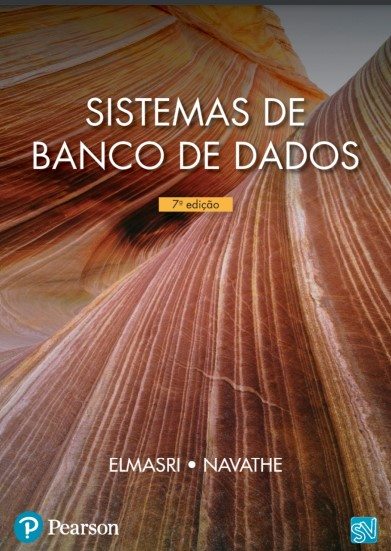
\includegraphics[scale=0.4]{Figuras/book.jpg}
\end{figure}
ELMASRI, R.; NAVATHE, S. B. Sistemas de Banco de Dados. 7. ed. São Paulo: Pearson Addison Wesley, 2019.
\end{ftst}


%==================================


\begin{ftst}{Fases do projeto de banco de dados}{Modelo Entidade-Relacionamento}
\begin{figure}
    \centering
    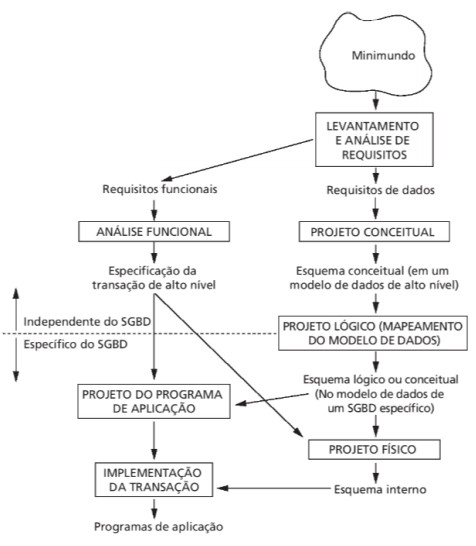
\includegraphics[scale=0.5]{Figuras/01_1.jpg}
\end{figure}

\end{ftst}

%==================================

\begin{ftst}{Introdução}{Modelo Entidade-Relacionamento}
\small
\vone
O Modelo Entidade-Relacionamento (MER) é um modelo de dados de alto-nível criado com o objetivo de representar a semântica associada aos dados do minimundo.
\vone 
20

O MER é utilizado para na fase de projeto conceitual, onde o esquema conceitual do
banco de dados da aplicação é concebido.
\vone
Seus conceitos são intuitivos, permitindo que projetistas de banco de dado capturem os conceitos associados aos dados da aplicação, sem a interferência da tecnologia específica de implementação do banco de dados. 
\vone
O esquema conceitual criado usando-se o MER é chamado \textbf{Diagrama Entidade Relacionamento (DER)}.

\end{ftst}

%==================================

\begin{ftst}{Entidades e Atributos}{Modelo Entidade-Relacionamento}
\small
\begin{itemize}
    \item O objeto mais elementar que o MER representa é a entidade. 
    \item Uma entidade é algo do mundo real que possui uma existência independente. 
    \begin{itemize}
        \item Objetos, pessoas ou conceitos do mundo real são representados como \textcolor{red}{Entidades}.
        \item Cada Entidade tem propriedades particulares que são chamadas de \textcolor{blue}{Atributos}.
        \begin{figure}
            \centering
            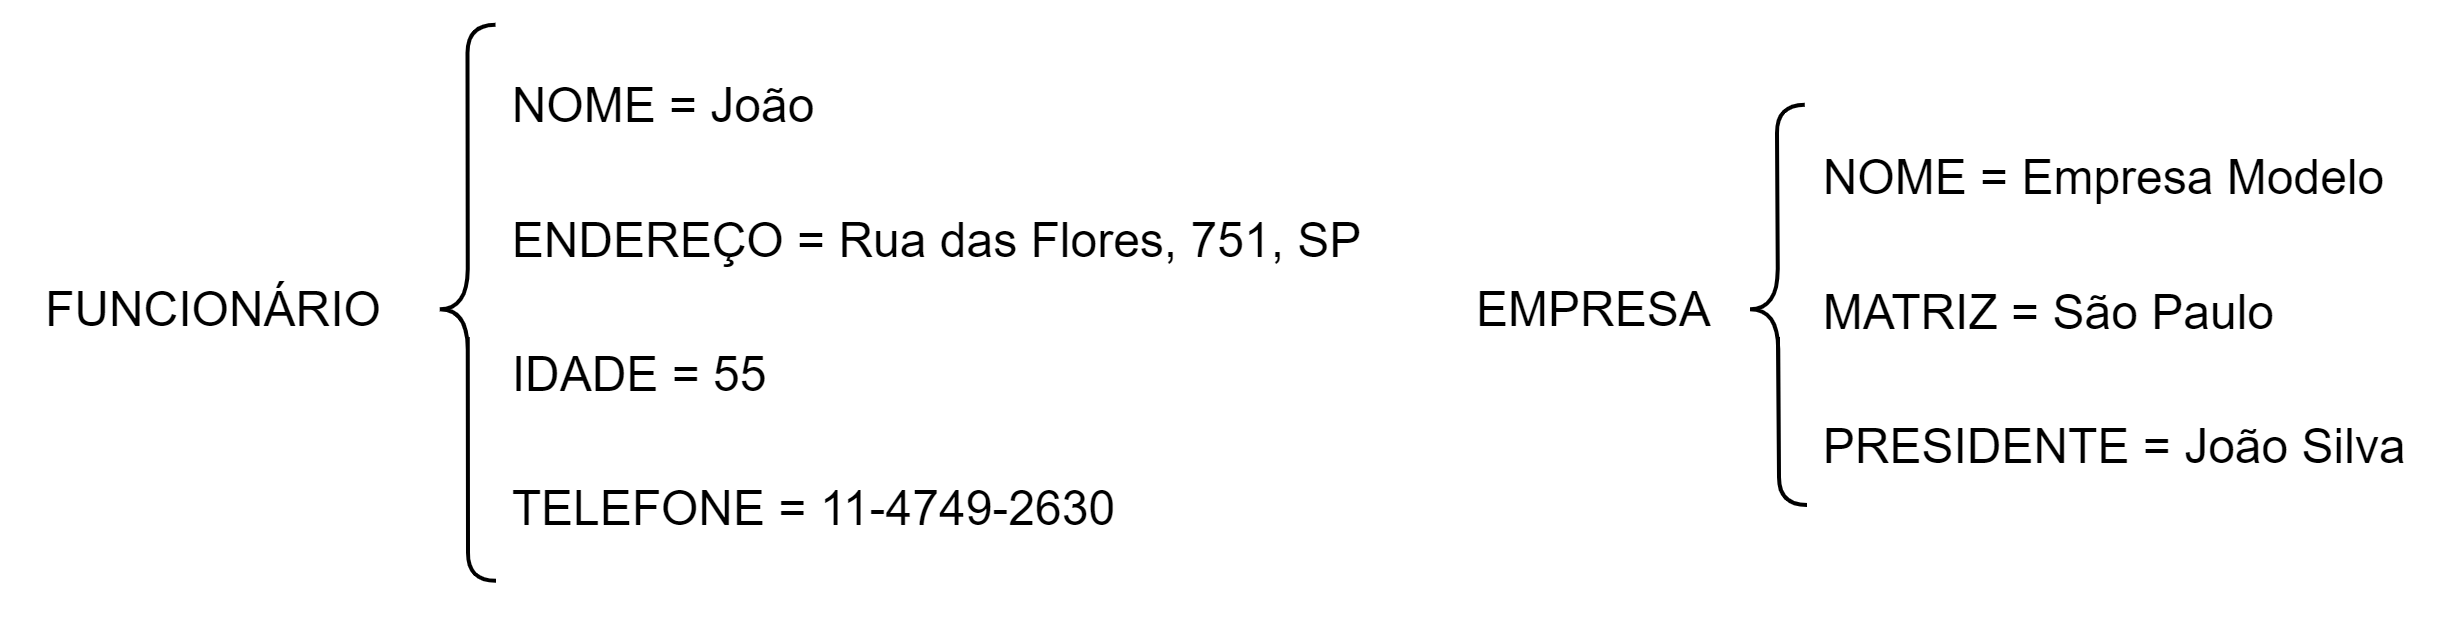
\includegraphics[scale=0.1]{Figuras/01_2.png}
        \end{figure}
        \item Representação no DER:
        \begin{figure}
            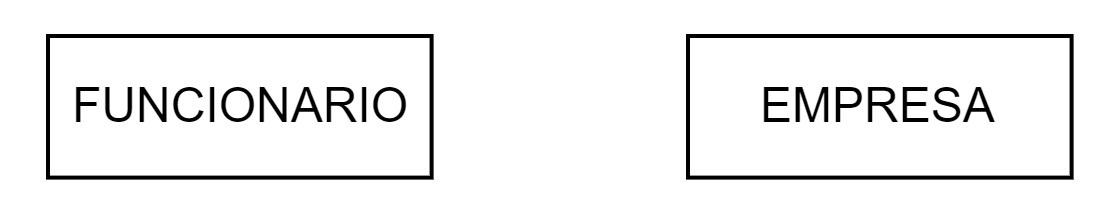
\includegraphics[scale=0.15]{Figuras/01_4.png}
        \end{figure}
    \end{itemize}

\end{itemize}


\end{ftst}

%==================================

\begin{ftst}{Atributos compostos versus simples}{Modelo Entidade-Relacionamento}
\small
\begin{itemize}
    \item \textbf{Atributos compostos} podem ser divididos em subpartes menores, que representam atributos mais básicos, com significados independentes. Exemplo: ENDERECO da entidade FUNCIONARIO.
    
    \item Os atributos compostos podem formar uma hierarquia. Exemplo: LOGRADOURO pode ser subdividido em três atributos simples: NUMERO, RUA e NUMERO\_APARTAMENTO.
    
    \item Os atributos não divisíveis são chamados \textbf{atributos simples ou atômicos}. 
\end{itemize}

\begin{figure}
    \centering
    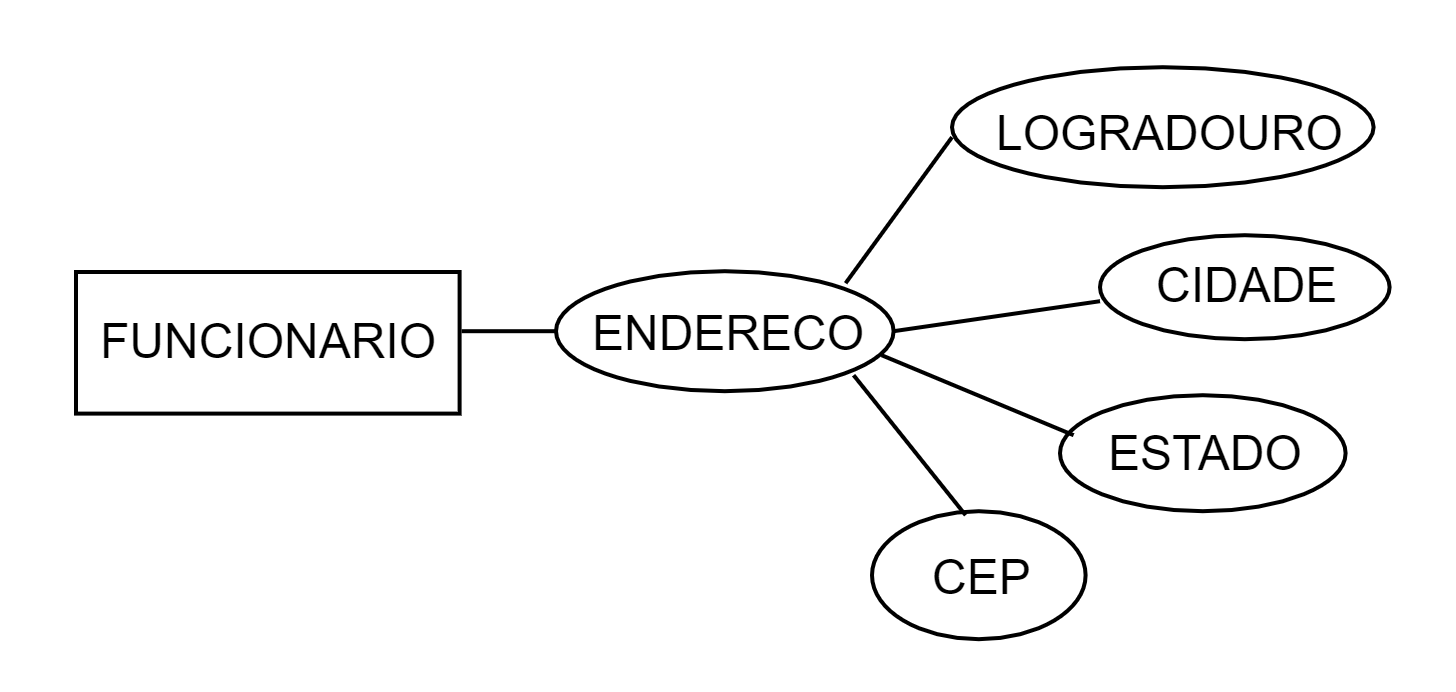
\includegraphics[scale=0.15]{Figuras/01_5.png}
\end{figure}

\end{ftst}

%==================================

\begin{ftst}{Atributos de valor único versus multivalorados}{Modelo Entidade-Relacionamento}
\small
\begin{itemize}
    \item \textbf{Atributos de valor único} possuem um valor único para uma entidade em particular. Exemplo: o atributo IDADE de uma FUNCIONARIO.
    
    \item Em alguns casos, um atributo pode ter um conjunto de valores para a mesma entidade. Esses atributos são chamados de \textbf{multivalorados}. Exemplo: FORMACAO\_ACADEMICA para uma pessoa.
    
    \item Um atributo multivalorado pode ter um limite mínimo e um máximo para restringir o número de valores permitidos para cada entidade individual. 
\end{itemize}
\begin{figure}
    \centering
    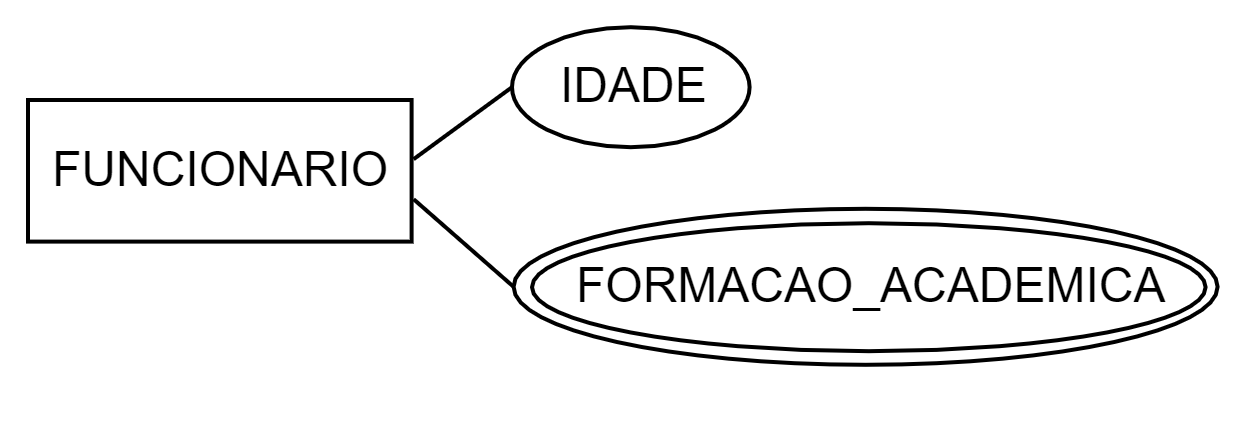
\includegraphics[scale=0.2]{Figuras/01_6.png}
\end{figure}

\end{ftst}

%==================================

\begin{ftst}{Atributos armazenados versus derivados}{Modelo Entidade-Relacionamento}
\small
Exemplo: para uma entidade de pessoa em particular, o valor do atributo Idade pode ser determinado pela data atual (hoje) e o valor do atributo Data\_nascimento dessa pessoa.
\vone
Nesse caso, o atributo Idade é chamado de \textbf{atributo derivado} e considerado derivável
do atributo Data\_nascimento, que é chamado, por sua vez, de \textbf{atributo armazenado}.
\vone
Alguns valores de atributo podem ser derivados de entidades relacionadas. Exemplo: um atributo Numero\_de\_funcionarios de uma entidade DEPARTAMENTO pode ser derivado contando-se o número de funcionários relacionados a esse departamento.

\begin{figure}
    \centering
    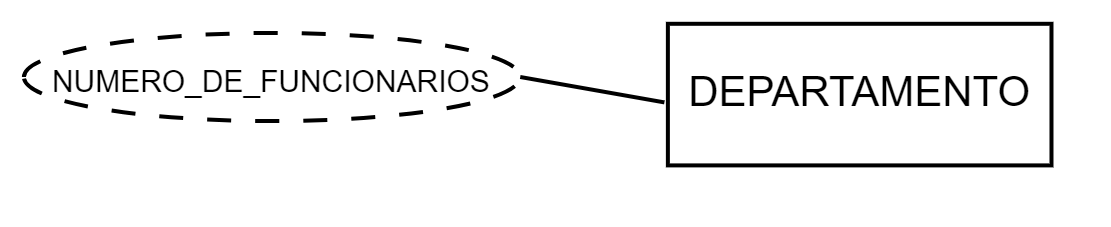
\includegraphics[scale=0.2]{Figuras/01_32.png}
\end{figure}

\end{ftst}

%==================================

\begin{ftst}{Valores NULL}{Modelo Entidade-Relacionamento}
\begin{itemize}
    \item Ocorre quando uma entidade em particular pode \textbf{não ter um valor aplicável} para um atributo ou esse valor é \textbf{desconhecido}.
    
    \item Exemplo de não aplicável: o atributo Numero\_apartamento de um endereço só se aplica a endereços que estão em prédios de apartamento, e não a outros tipos de residências, como casas.
    
    \item A categoria desconhecido ainda pode ser classificada em mais dois casos:
    \begin{itemize}
        \item O primeiro caso acontece quando se sabe que o valor do atributo existe, mas está faltando. Exemplo: se o atributo Altura de uma pessoa for listado como NULL.
        \item O segundo caso surge quando não se sabe se o valor do atributo existe. Exemplo: se o atributo Telefone\_residencial de uma pessoa for NULL.
    \end{itemize} 
\end{itemize}


\end{ftst}

%==================================

\begin{ftst}{Atributos-chave de um tipo de entidade}{Modelo Entidade-Relacionamento}
\small
\begin{itemize}
    \item Um \textbf{atributo-chave} é usado para identificar cada entidade de maneira exclusiva. Exemplo: Para o tipo de entidade FUNCIONARIO, um atributo-chave típico é o CPF (Cadastro de Pessoa Física), pois duas pessoas não podem ter o mesmo CPF.
    
    \item Às vezes, vários atributos juntos formam uma chave,significando que a combinação dos valores de atributo deve ser distinta para cada entidade.\textit{ Nesses casos, teremos um atributo composto que é um atributo-chave.}
    
    \item \textbf{As chaves compostas devem ser mínimas!}
    \begin{figure}
        \centering
        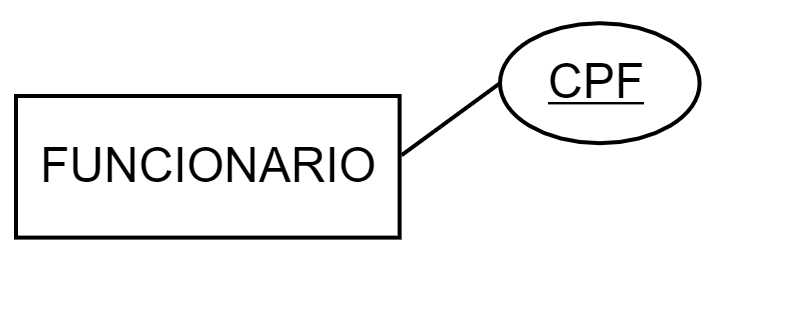
\includegraphics[scale=0.2]{Figuras/01_7.png}
    \end{figure}
\end{itemize}

\end{ftst}

%==================================

\begin{ftst}{Relacionamentos}{Modelo Entidade-Relacionamento}

\begin{itemize}
    \item Um relacionamento é uma associação entre uma ou mais entidades.
\end{itemize}

\begin{figure}
    \centering
    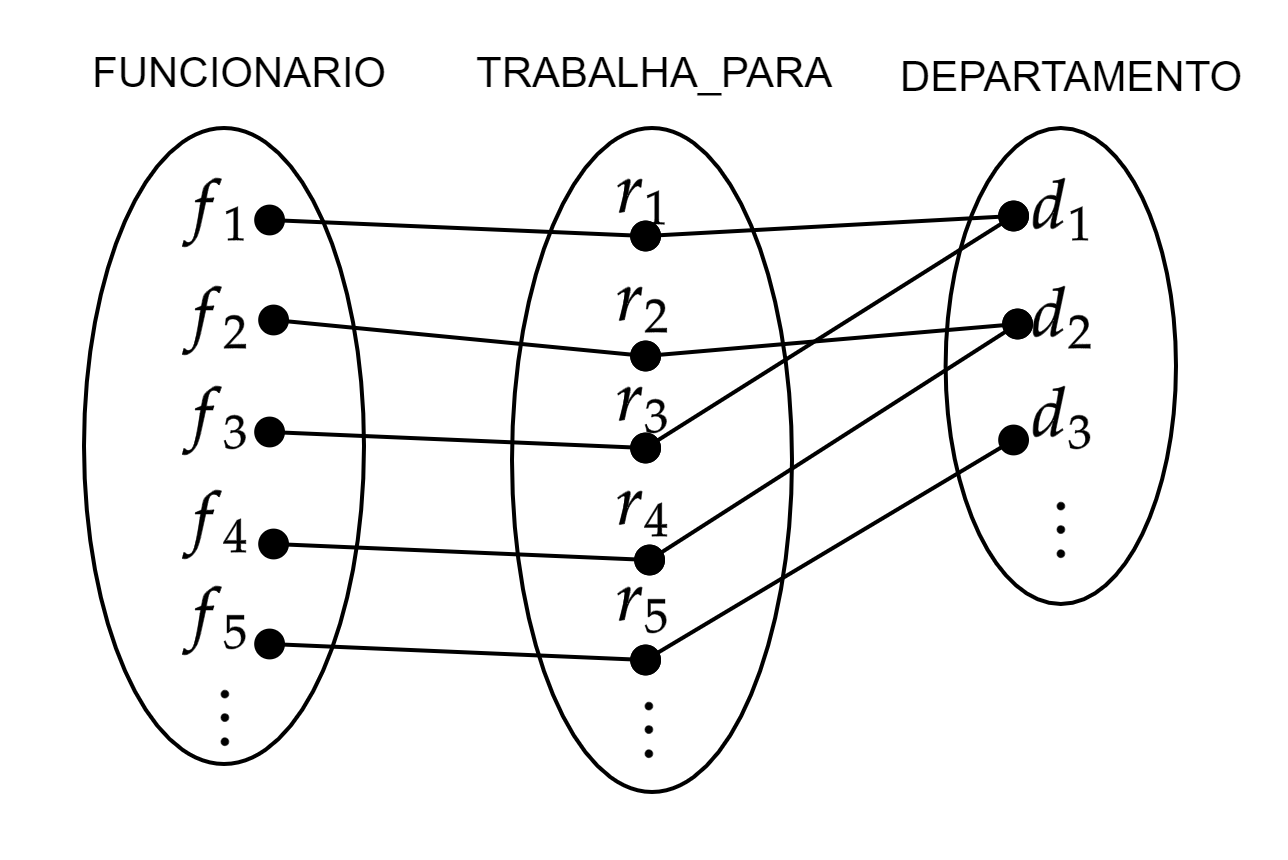
\includegraphics[scale=0.2]{Figuras/01_8.png}
\end{figure}

\end{ftst}

%==================================

\begin{ftst}{Grau de um relacionamentos}{Modelo Entidade-Relacionamento}
\small
\begin{itemize}
    \item O grau de um tipo de relacionamento é o número de entidades participantes.
    \item Relacionamentos entre duas entidades são de grau 2 e são chamados de \textbf{binários}. Exemplo: TRABALHA\_PARA.
    \item Relacionamentos com grau três é chamado \textbf{ternário}.
\end{itemize}

\begin{figure}
    \centering
    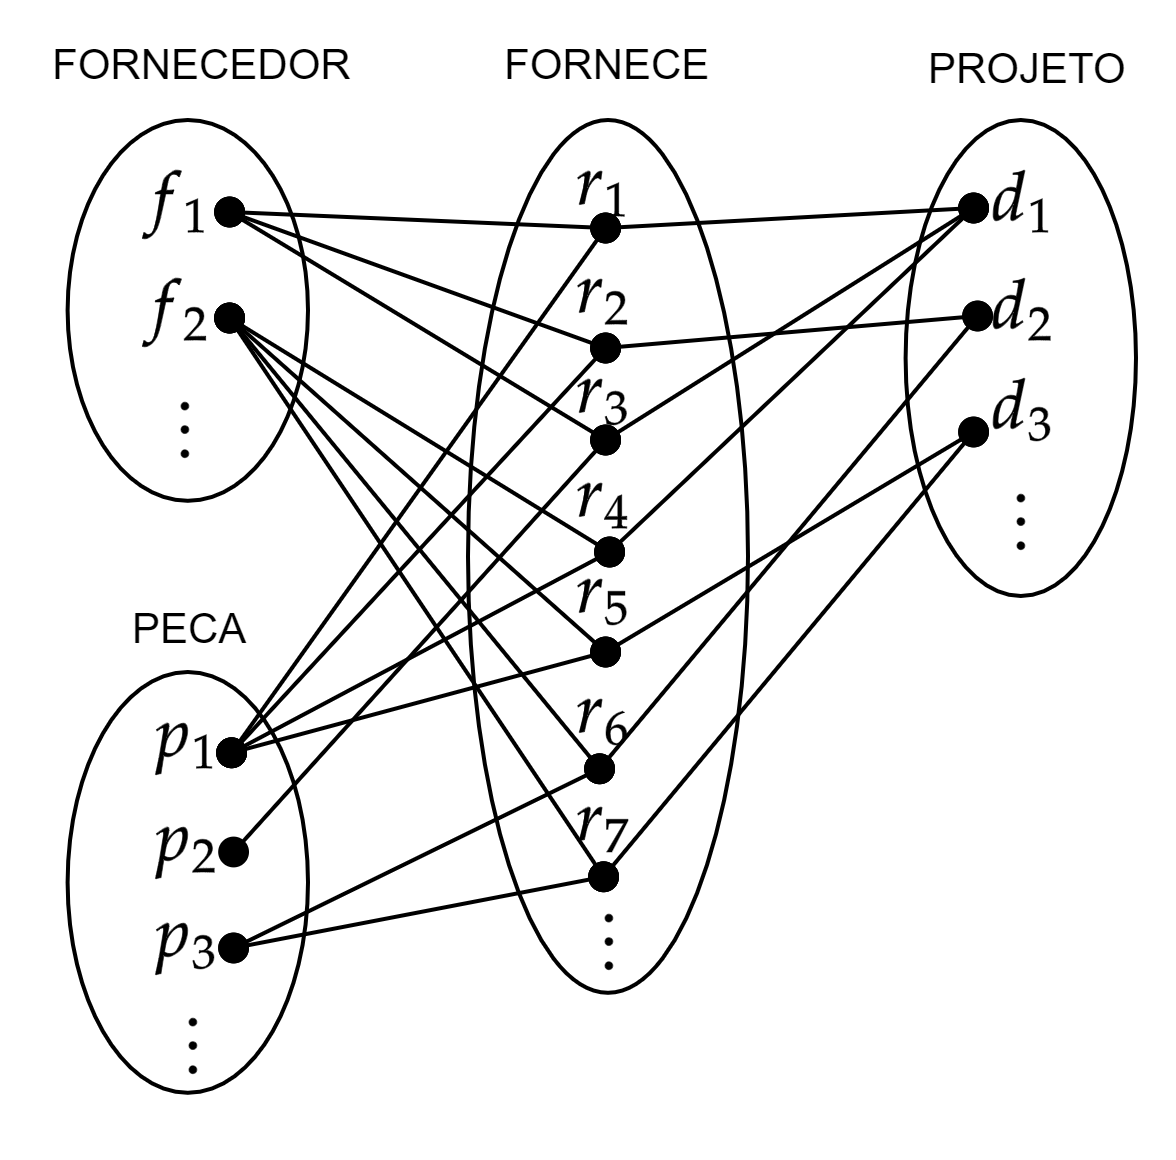
\includegraphics[scale=0.12]{Figuras/01_9.png}
\end{figure}

\end{ftst}

%==================================

\begin{ftst}{Grau de um relacionamentos}{Modelo Entidade-Relacionamento}
\small
\begin{itemize}
    \item O grau de um tipo de relacionamento é o número de entidades participantes.
    \item Relacionamentos entre duas entidades são de grau 2 e são chamados de \textbf{binários}. Exemplo: TRABALHA\_PARA.
    \item Relacionamentos com grau três é chamado \textbf{ternário}.
\end{itemize}

\begin{figure}
    \centering
    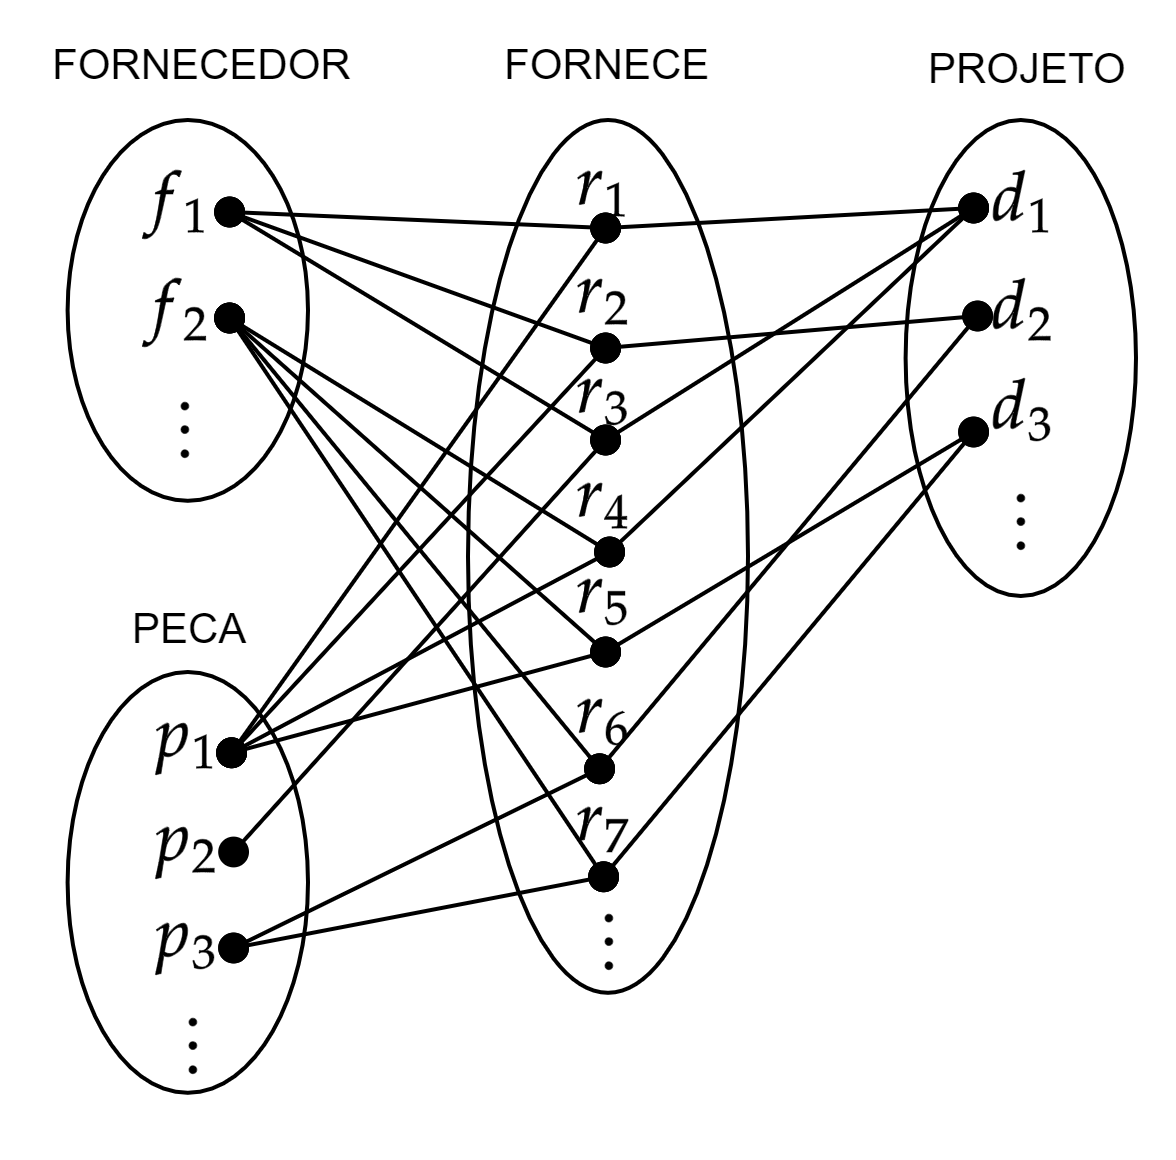
\includegraphics[scale=0.12]{Figuras/01_9.png}
\end{figure}

\end{ftst}

%==================================

\begin{ftst}{Grau de um relacionamentos}{Modelo Entidade-Relacionamento}
\begin{itemize}
    \item Representação no DER.
\end{itemize}
\vone
\begin{figure}
    \centering
    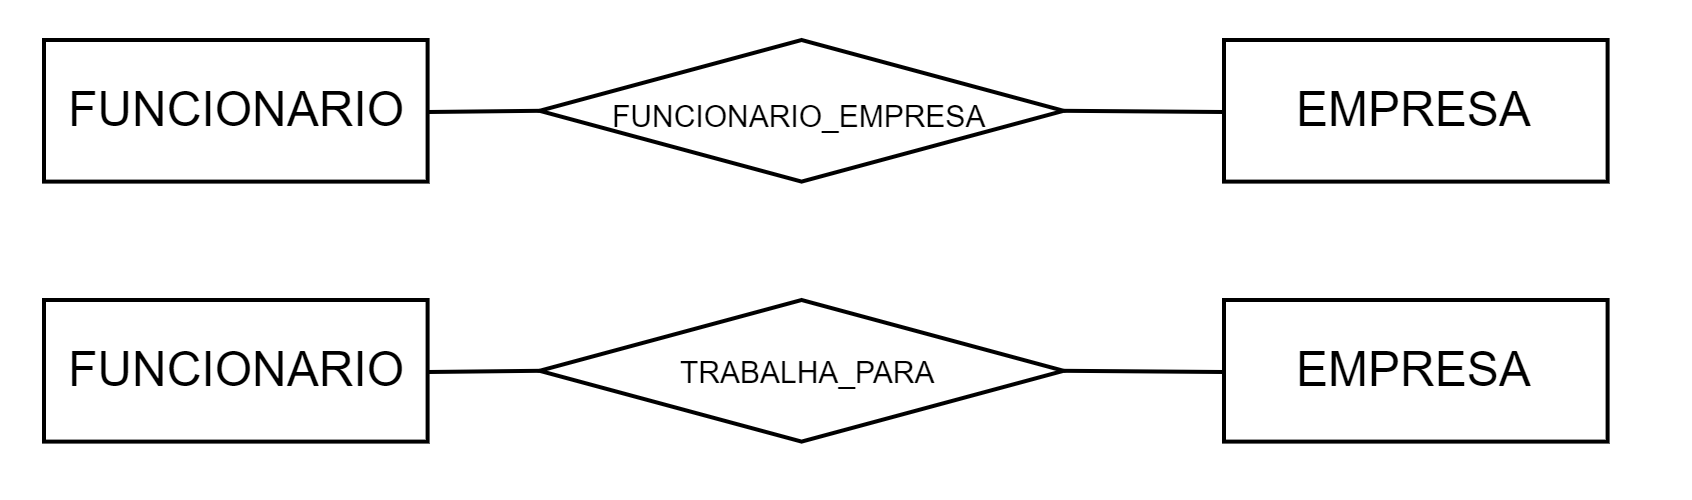
\includegraphics[scale=0.2]{Figuras/01_10.png}
\end{figure}

\end{ftst}

%==================================

\begin{ftst}{Papéis}{Modelo Entidade-Relacionamento}
\begin{itemize}
    \item Papel é a função que uma ocorrência da entidade cumpre dentro de uma ocorrência do relacionamento.
    \item Não é obrigatória no DER.
\end{itemize}
\vone
\begin{figure}
    \centering
    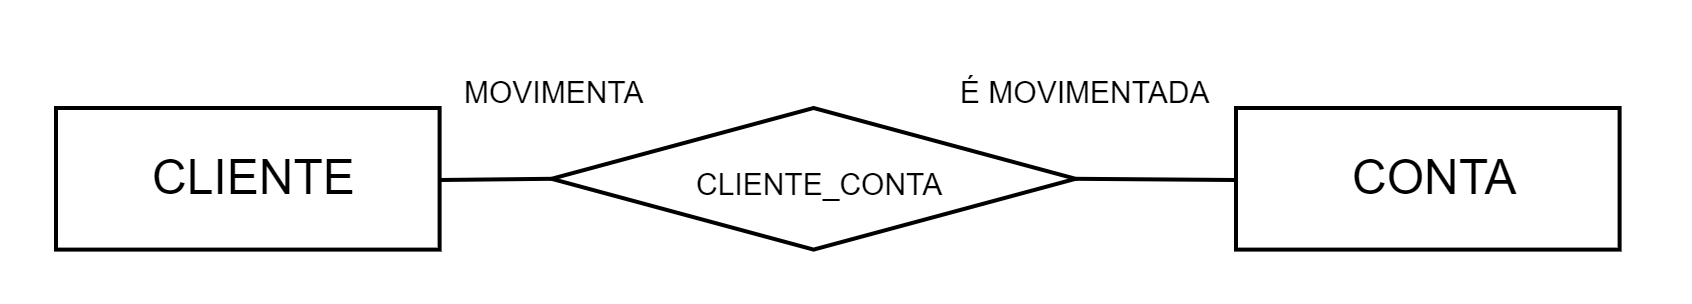
\includegraphics[scale=0.2]{Figuras/01_11.png}
\end{figure}

\end{ftst}

%==================================

\begin{ftst}{Relacionamentos Recursivos ou Autorrelacionamento}{Modelo Entidade-Relacionamento}
\begin{itemize}
    \item Quando a mesma entidade participa mais de uma vez em um relacionamento em papéis diferentes.
    \item Nesse caso, o uso dos papéis é recomendado.
\end{itemize}
\vone
\begin{figure}
    \centering
    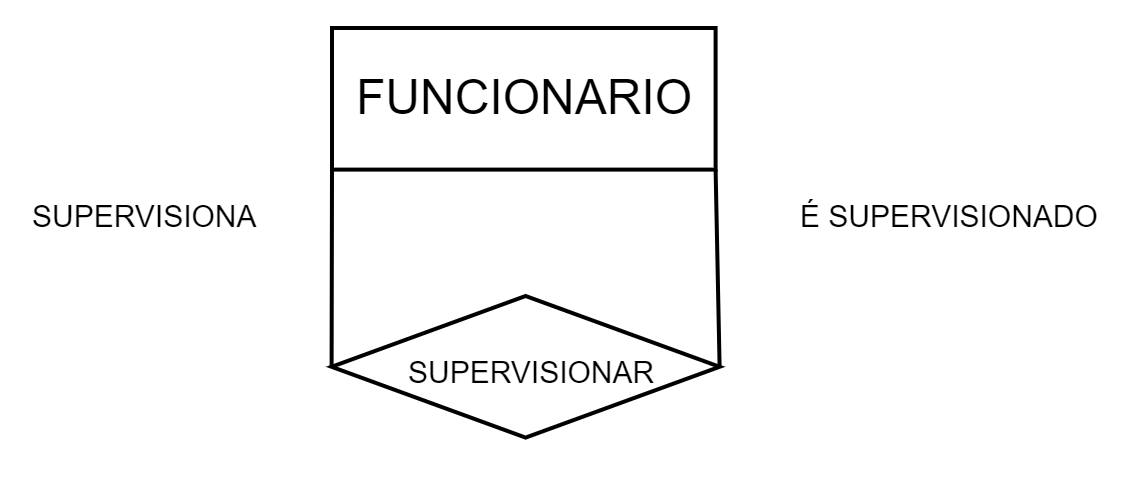
\includegraphics[scale=0.25]{Figuras/01_12.png}
\end{figure}

\end{ftst}

%==================================

\begin{ftst}{Restrições sobre tipos de relacionamento binários}{Modelo Entidade-Relacionamento}
\begin{itemize}
    \item Os tipos de relacionamento costumam ter certas restrições que limitam as combinações de entidades que podem participar no conjunto de relacionamentos correspondente.
    \item Essas restrições são determinadas com base na situação do minimundo que os relacionamentos representam. 
    \item Exemplo: se a empresa tem uma regra de que cada funcionário precisa trabalhar para exatamente um departamento, precisamos descrever essa restrição no DER.
    \item Os dois tipos principais de restrições de relacionamento binário são \textbf{razão de
cardinalidade} e \textbf{participação}.
\end{itemize}


\end{ftst}

%==================================

\begin{ftst}{Razões de cardinalidade para relacionamentos binários}{Modelo Entidade-Relacionamento}
\begin{itemize}
    \item Cardinalidade (mínima, máxima) de uma entidade em um relacionamento é o número (mínimo, máximo) de ocorrências de entidade associadas a uma ocorrência da entidade em questão através do relacionamento.
    \item As razões de cardinalidade possíveis para tipos de relacionamento binários são 1:1, 1:N, N:1 e M:N.
\end{itemize}
\begin{figure}
    \centering
    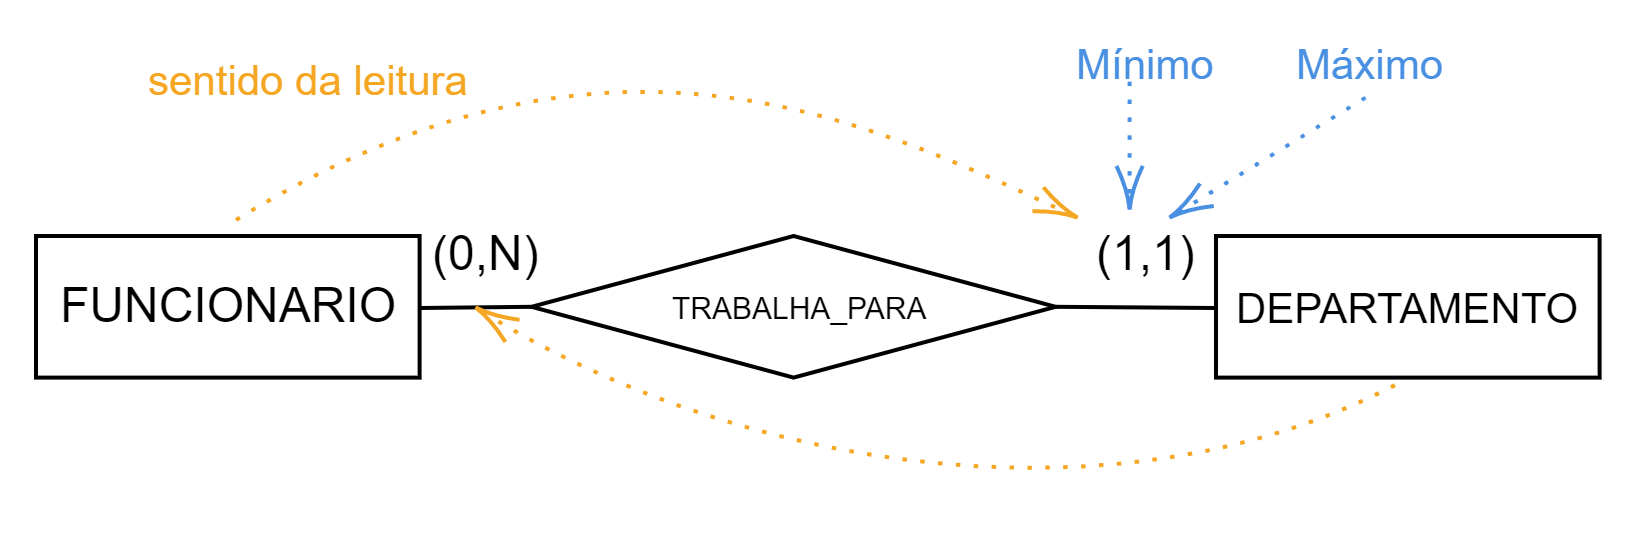
\includegraphics[scale=0.2]{Figuras/01_13.png}
\end{figure}
\end{ftst}

%==================================

\begin{ftst}{Relacionamento Um para Um – 1:1}{Modelo Entidade-Relacionamento}
\begin{itemize}
    \item Uma ocorrência de \textbf{A} está associada a \textbf{no máximo uma} ocorrência de \textbf{B}, e uma ocorrência em \textbf{B} está associada a \textbf{no máximo uma} ocorrência em \textbf{A}.
\end{itemize}
\begin{figure}
    \centering
    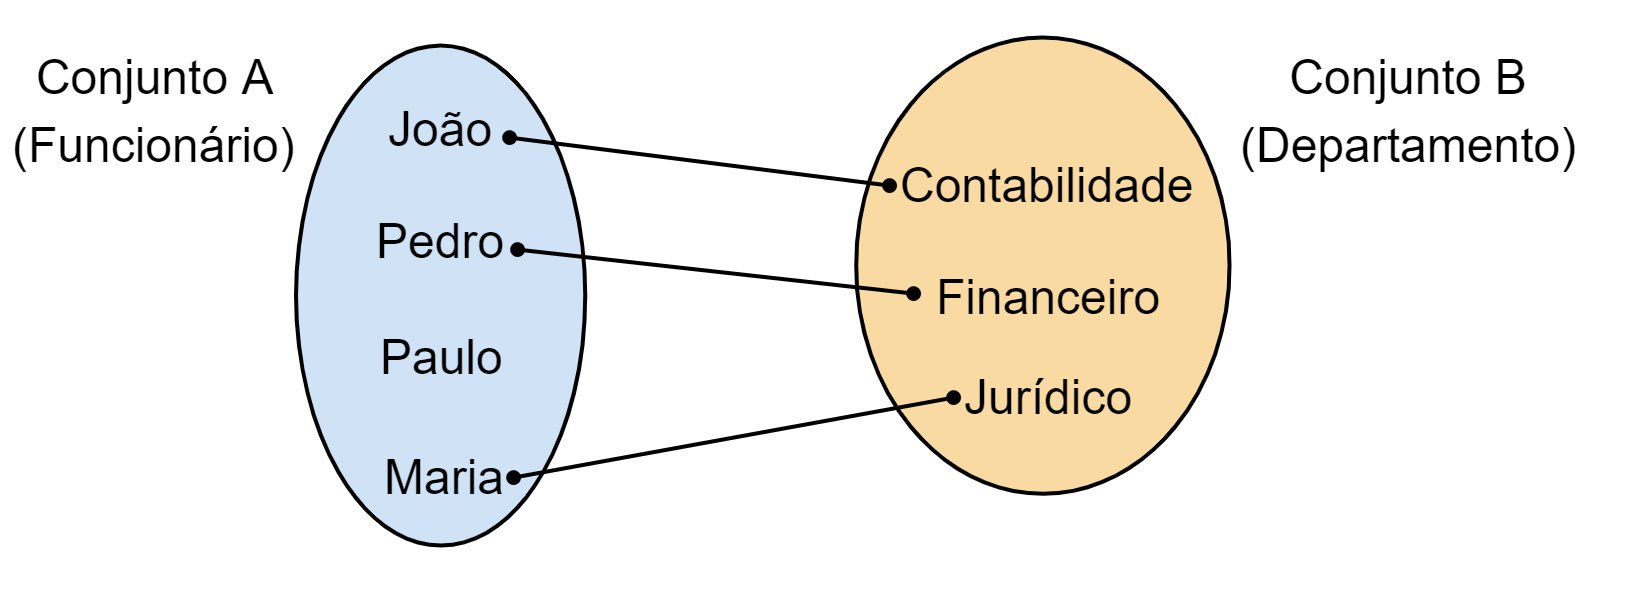
\includegraphics[scale=0.15]{Figuras/01_15.png}
\end{figure}
\begin{figure}
    \centering
    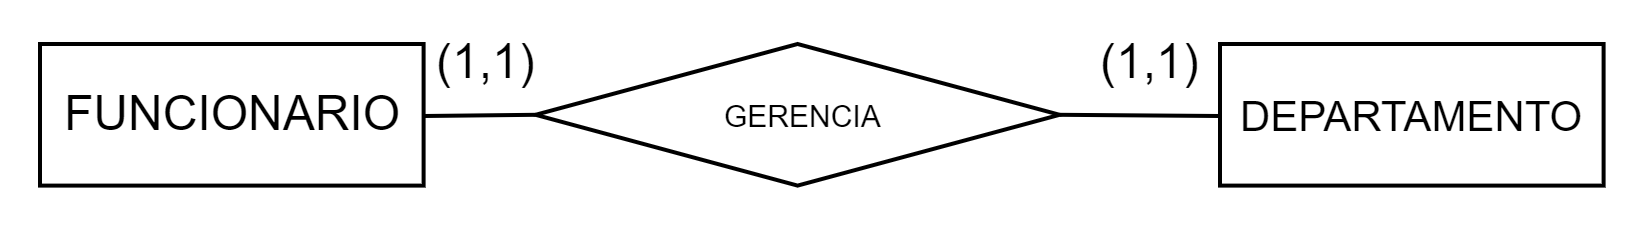
\includegraphics[scale=0.2]{Figuras/01_14.png}
\end{figure}


\end{ftst}

%==================================

\begin{ftst}{Relacionamento Um para Muitos – 1:N}{Modelo Entidade-Relacionamento}
\begin{itemize}
    \item Uma ocorrência de \textbf{A} está associada a \textbf{várias} ocorrências de \textbf{B}, porém uma ocorrência de \textbf{B} deve estar associada a \textbf{no máximo uma} ocorrência em \textbf{A}.
\end{itemize}
\begin{figure}
    \centering
    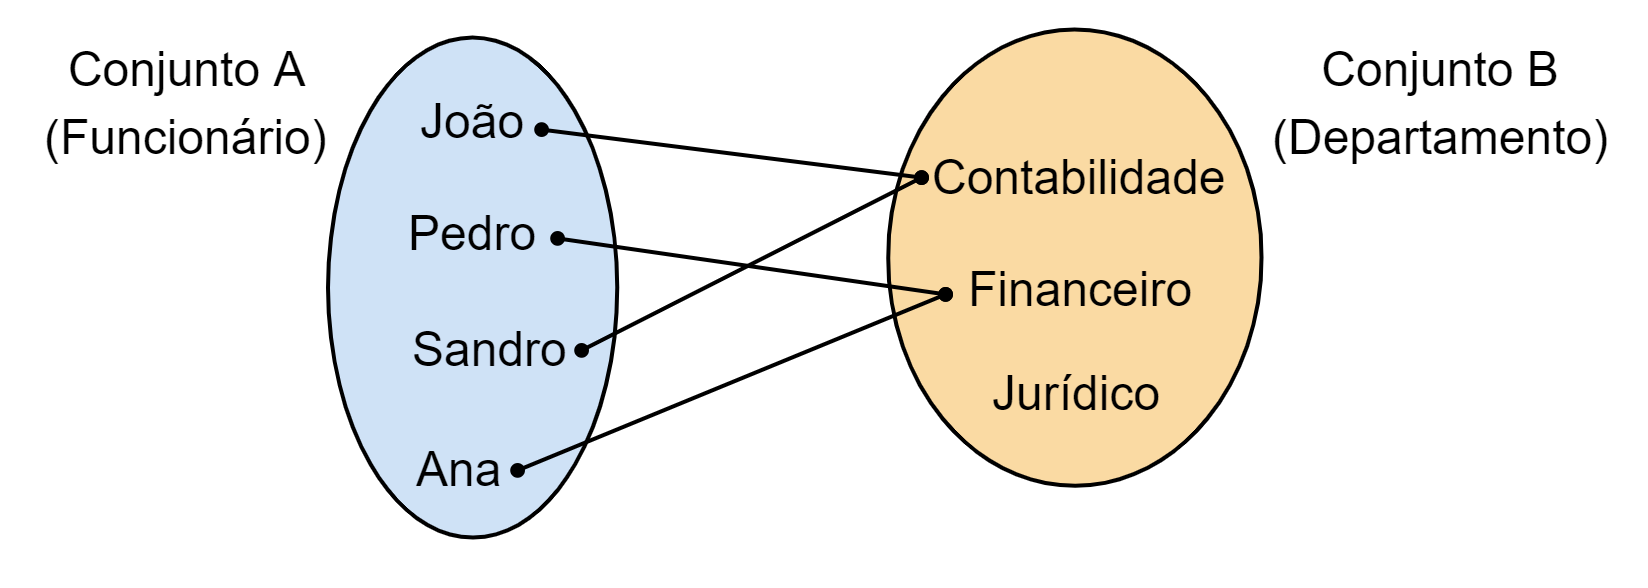
\includegraphics[scale=0.15]{Figuras/01_17.png}
\end{figure}
\begin{figure}
    \centering
    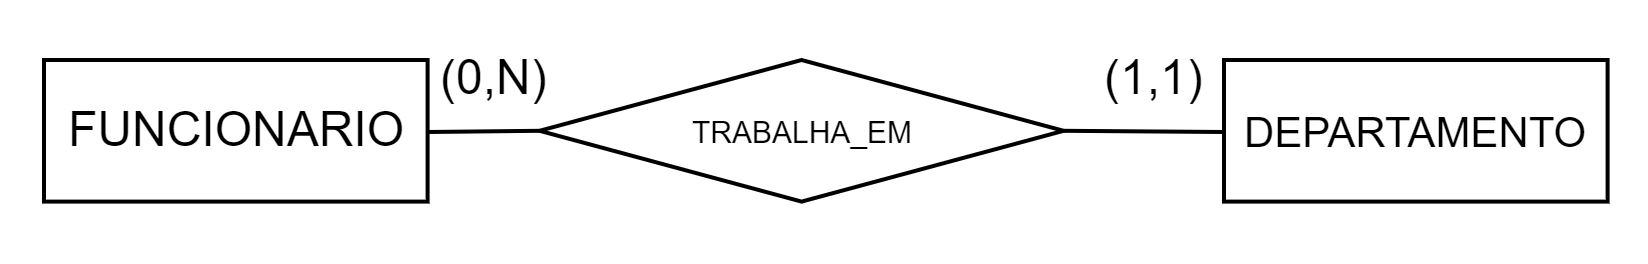
\includegraphics[scale=0.2]{Figuras/01_16.png}
\end{figure}


\end{ftst}

%==================================

\begin{ftst}{Relacionamento Muitos para Muitos – M:N ou N:N}{Modelo Entidade-Relacionamento}
\begin{itemize}
    \item Uma ocorrência de \textbf{A} está associada a \textbf{qualquer} número de ocorrências de \textbf{B}, uma ocorrência de \textbf{B} está associada a \textbf{qualquer número} de ocorrências em \textbf{A}.
\end{itemize}
\begin{figure}
    \centering
    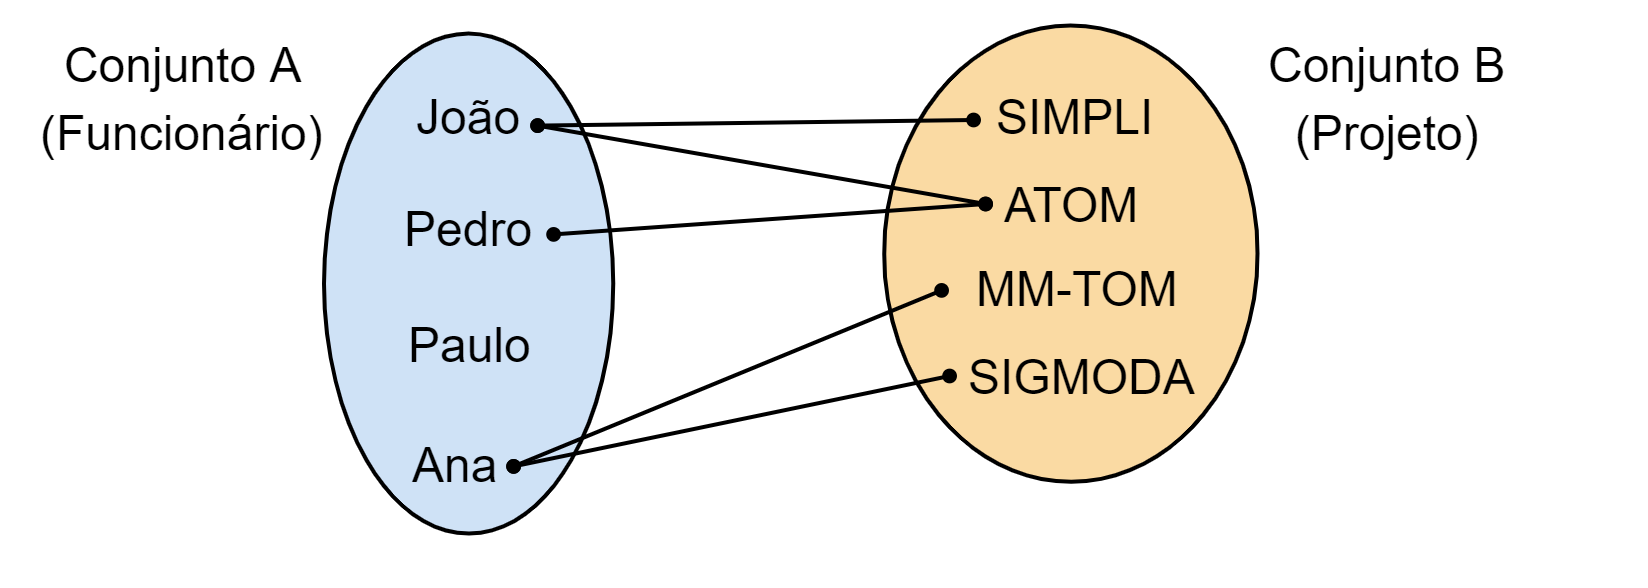
\includegraphics[scale=0.15]{Figuras/01_19.png}
\end{figure}
\begin{figure}
    \centering
    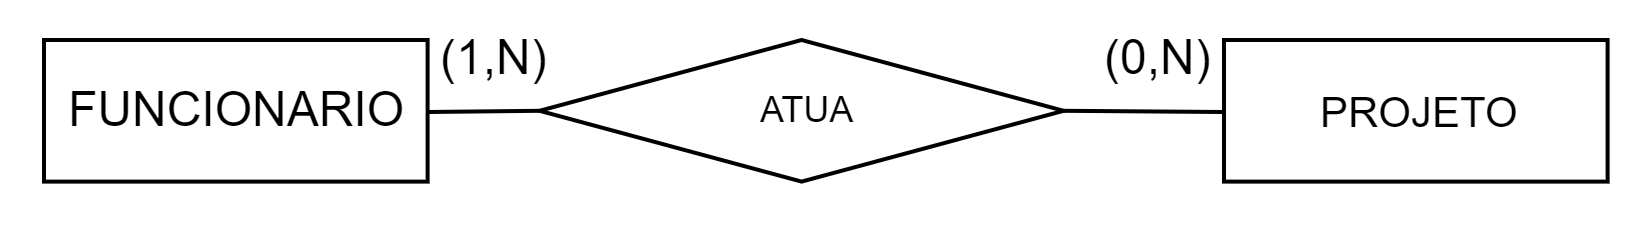
\includegraphics[scale=0.2]{Figuras/01_18.png}
\end{figure}
\end{ftst}

%==================================

\begin{ftst}{\large Restrições de participação e dependência de existência}{Modelo Entidade-Relacionamento}
\footnotesize
\begin{itemize}
    \item A restrição de participação especifica se a existência de uma entidade depende de ela estar relacionada a outra entidade por meio do tipo de relacionamento.
    \item Existem dois tipos de restrições de participação: \textbf{total }e \textbf{parcial}.
    \item \textbf{Exemplo de participação total:} Se a política de uma empresa afirma que todo funcionário precisa trabalhar para um departamento, uma entidade de funcionário só pode existir se participar em, pelo menos, uma instância de relacionamento. 
    \item Assim, a participação de FUNCIONÁRIO no relacionamento TRABALHA\_EM é chamada de \textbf{participação total}, também conhecida como \textbf{dependência de existência}.
    \item Notação: linha dupla.
\end{itemize}

\begin{figure}
    \centering
    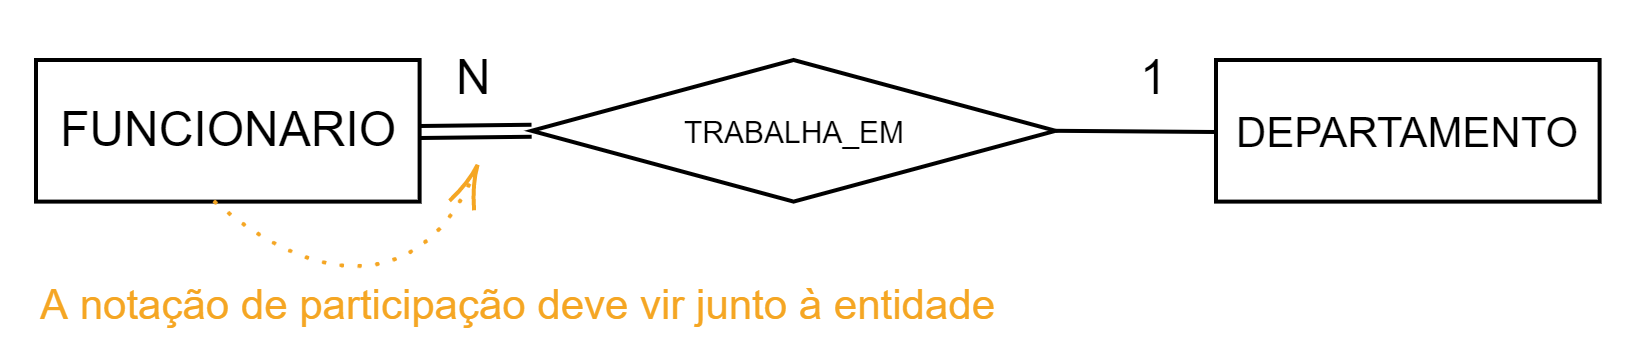
\includegraphics[scale=0.2]{Figuras/01_20.png}
\end{figure}


\end{ftst}

%==================================

\begin{ftst}{\large Restrições de participação e dependência de existência}{Modelo Entidade-Relacionamento}
\begin{itemize}
    \item \textbf{Exemplo de participação parcial:} a participação de DEPARTAMENTO no relacionamento TRABALHA\_EM, significando que uma parte do conjunto de entidades de DEPARTAMENTO está relacionada a alguma entidade de FUNCIONÁRIO por meio de TRABALHA\_EM, mas não necessariamente todas.
    \item Notação: linha simples.
\end{itemize}

\begin{figure}
    \centering
    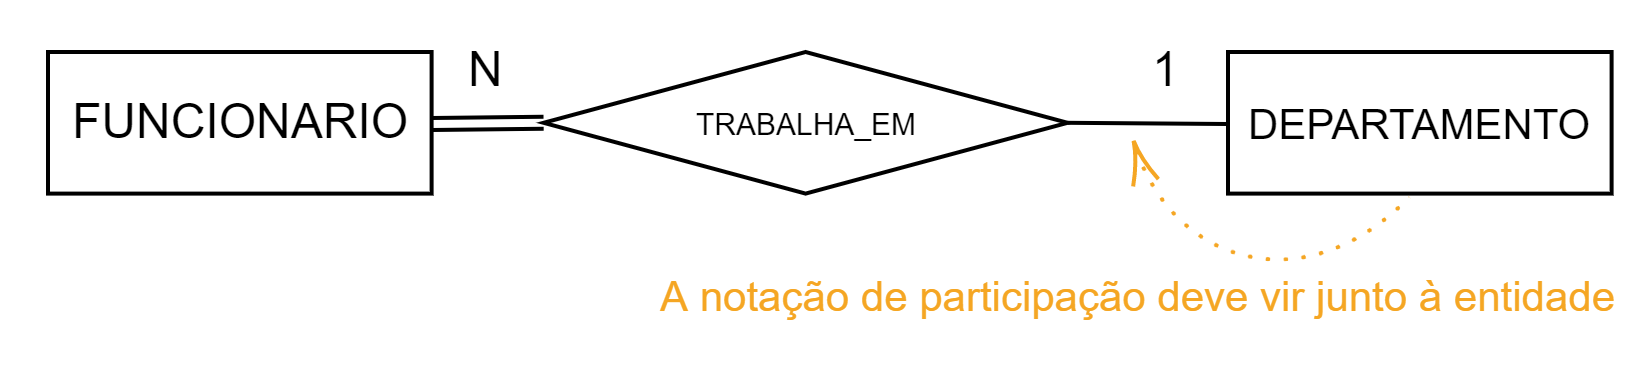
\includegraphics[scale=0.2]{Figuras/01_21.png}
\end{figure}


\end{ftst}

%==================================

\begin{ftst}{Atributos de relacionamento}{Modelo Entidade-Relacionamento}
\begin{itemize}
    \item Os relacionamentos também podem ter atributos, semelhantes àqueles de entidade.
    \item Exemplo: para registrar o número de horas por semana que um funcionário trabalha em um determinado projeto, podemos incluir um atributo HORAS para o relacionamento ATUA.
\end{itemize}
\vone
\begin{figure}
    \centering
    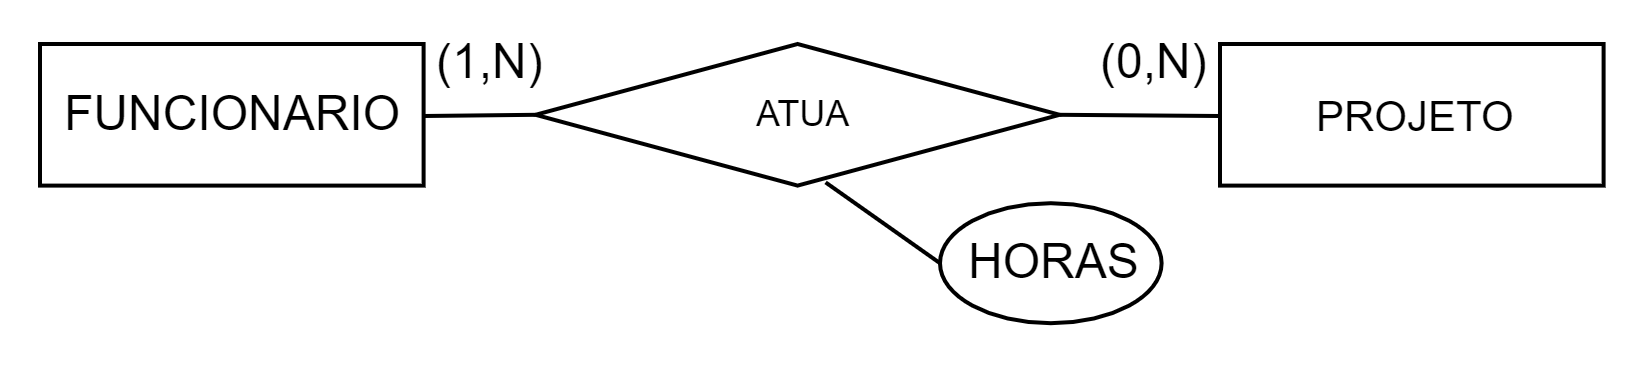
\includegraphics[scale=0.2]{Figuras/01_22.png}
\end{figure}


\end{ftst}

%==================================

\begin{ftst}{Entidade fraca}{Modelo Entidade-Relacionamento}
\small
\begin{itemize}
    \item Entidade que não possuem atributos-chave próprios são chamadas de \textbf{entidade fraca}.
    \item Ao contrário, as entidades regulares que possuem um atributo-chave, que incluem todos os exemplos discutidos até aqui —são chamadas de \textbf{entidade forte}.
    \item Entidades fortes que se relacionam com entidades fracas são chamadas de entidades \textbf{proprietárias} ou entidades \textbf{de identificação}.
    \item Os relacionamentos que relacionam entidades proprietárias e entidades fracas são chamados de \textbf{relacionamentos de identificação.}
    \item Uma entidade fraca sempre tem uma restrição de participação total (dependência de existência) com relação a seu relacionamento de identificação, porque a entidade fraca não pode ser identificada sem uma entidade proprietária.
\end{itemize}
\end{ftst}

%==================================

\begin{ftst}{Entidade fraca}{Modelo Entidade-Relacionamento}
\small
\begin{itemize}
    \item Um tipo de entidade fraca normalmente tem uma \textbf{chave parcial}, que é o atributo que pode identificar exclusivamente as entidades fracas que estão relacionadas à mesma entidade proprietária.
    \item Em diagramas ER, tanto um tipo de entidade fraca quanto seu relacionamento de identificação são distinguidos com linhas duplas. 
    \item O atributo de chave parcial é sublinhado com uma linha tracejada ou pontilhada.
\end{itemize}

\begin{figure}
    \centering
    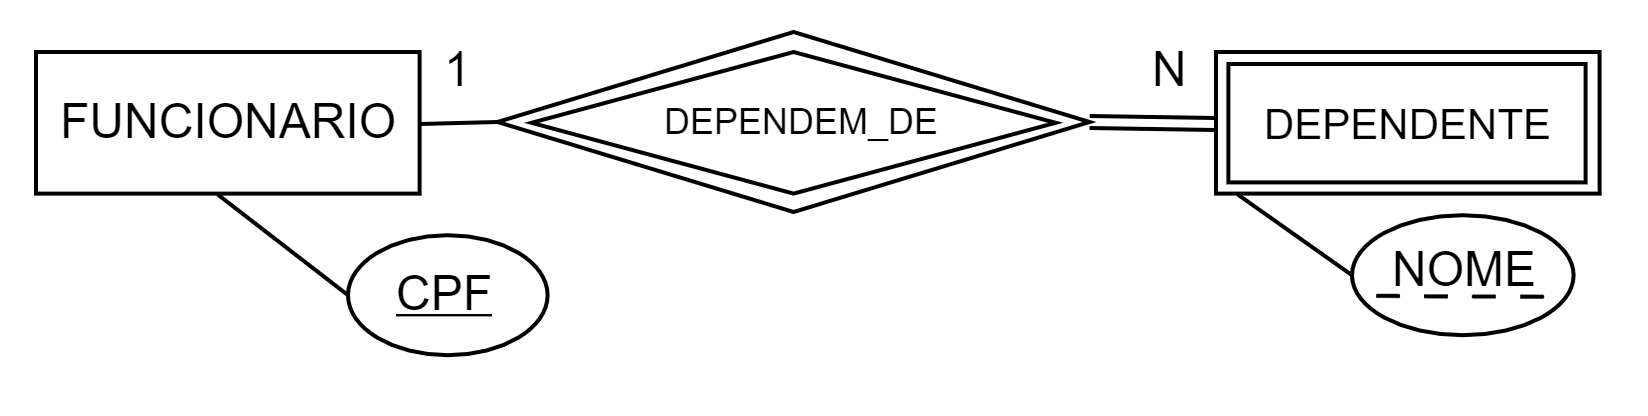
\includegraphics[scale=0.2]{Figuras/01_23.png}
\end{figure}


\end{ftst}

%==================================

\begin{ftst}{Tipos de relacionamento de grau maior que dois}{Modelo Entidade-Relacionamento}
\begin{itemize}
    \item O grau de um relacionamento é o número de entidades participantes. Chamamos um relacionamento de grau dois de \textbf{binário}, de grau três de \textbf{ternário} e de \textbf{n-ários} os demais.
    \item A notação é a mesma.
\end{itemize}

\begin{figure}
    \centering
    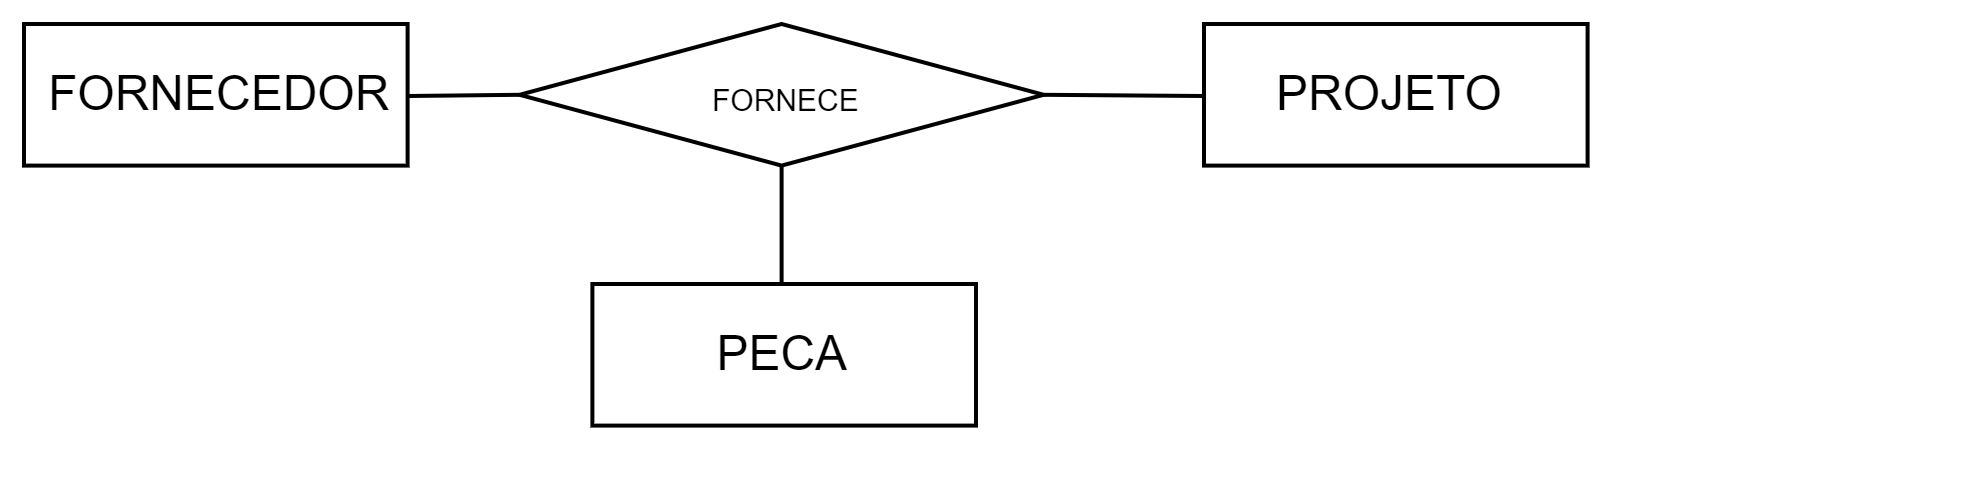
\includegraphics[scale=0.2]{Figuras/01_24.png}
\end{figure}

\end{ftst}

%==================================

\begin{ftst}{Restrições sobre relacionamentos ternários
(ou n-ários)}{Modelo Entidade-Relacionamento}
\begin{itemize}
    \item A leitura é feita \textbf{par a par}.
\end{itemize}

\begin{figure}
    \centering
    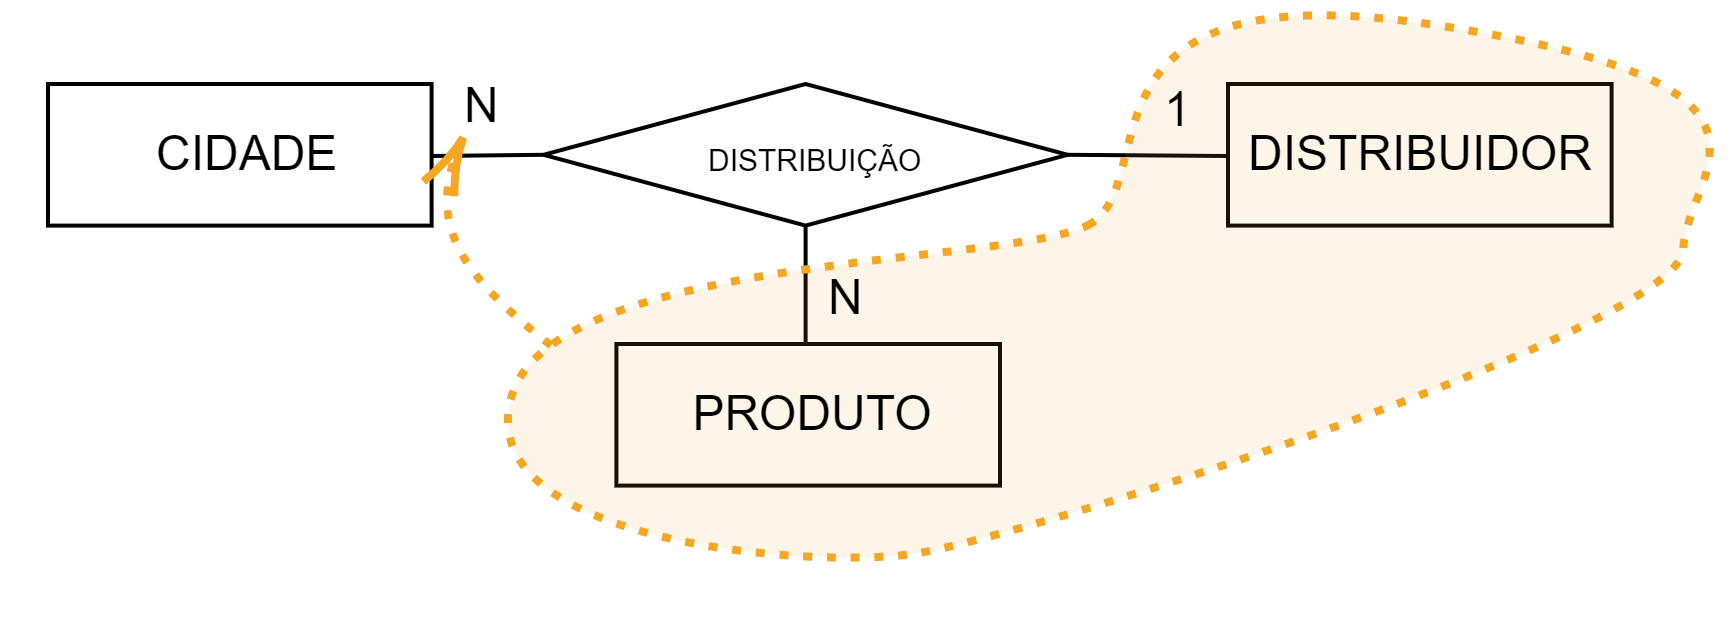
\includegraphics[scale=0.2]{Figuras/01_26.png}
\end{figure}

\end{ftst}

%==================================

\begin{ftst}{Restrições sobre relacionamentos ternários
(ou n-ários)}{Modelo Entidade-Relacionamento}

\begin{figure}
    \centering
    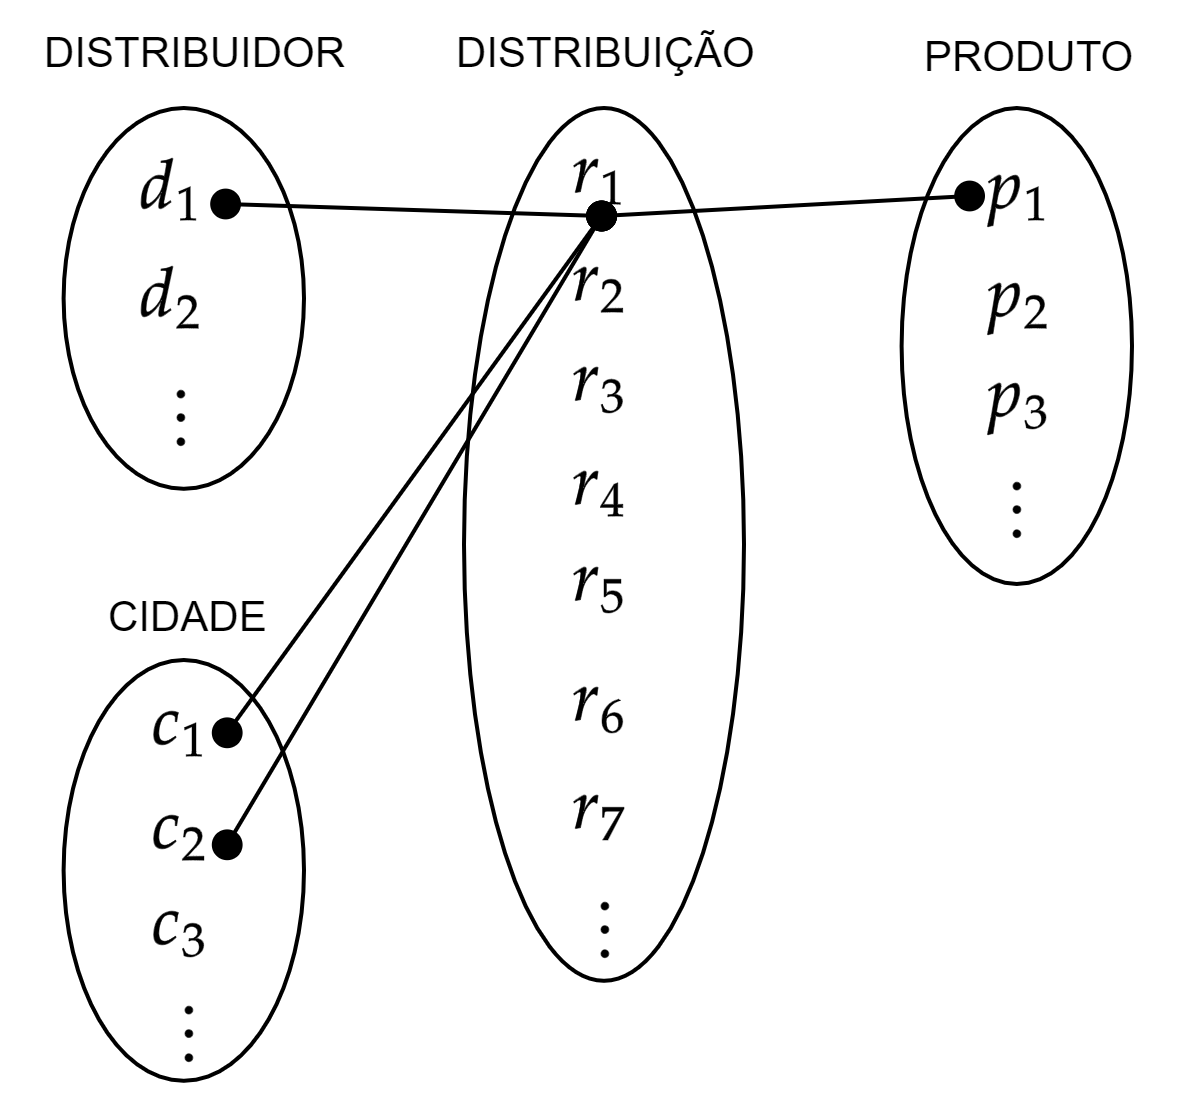
\includegraphics[scale=0.16]{Figuras/01_29.png}
\end{figure}

\end{ftst}

%==================================

\begin{ftst}{Restrições sobre relacionamentos ternários
(ou n-ários)}{Modelo Entidade-Relacionamento}

\begin{figure}
    \centering
    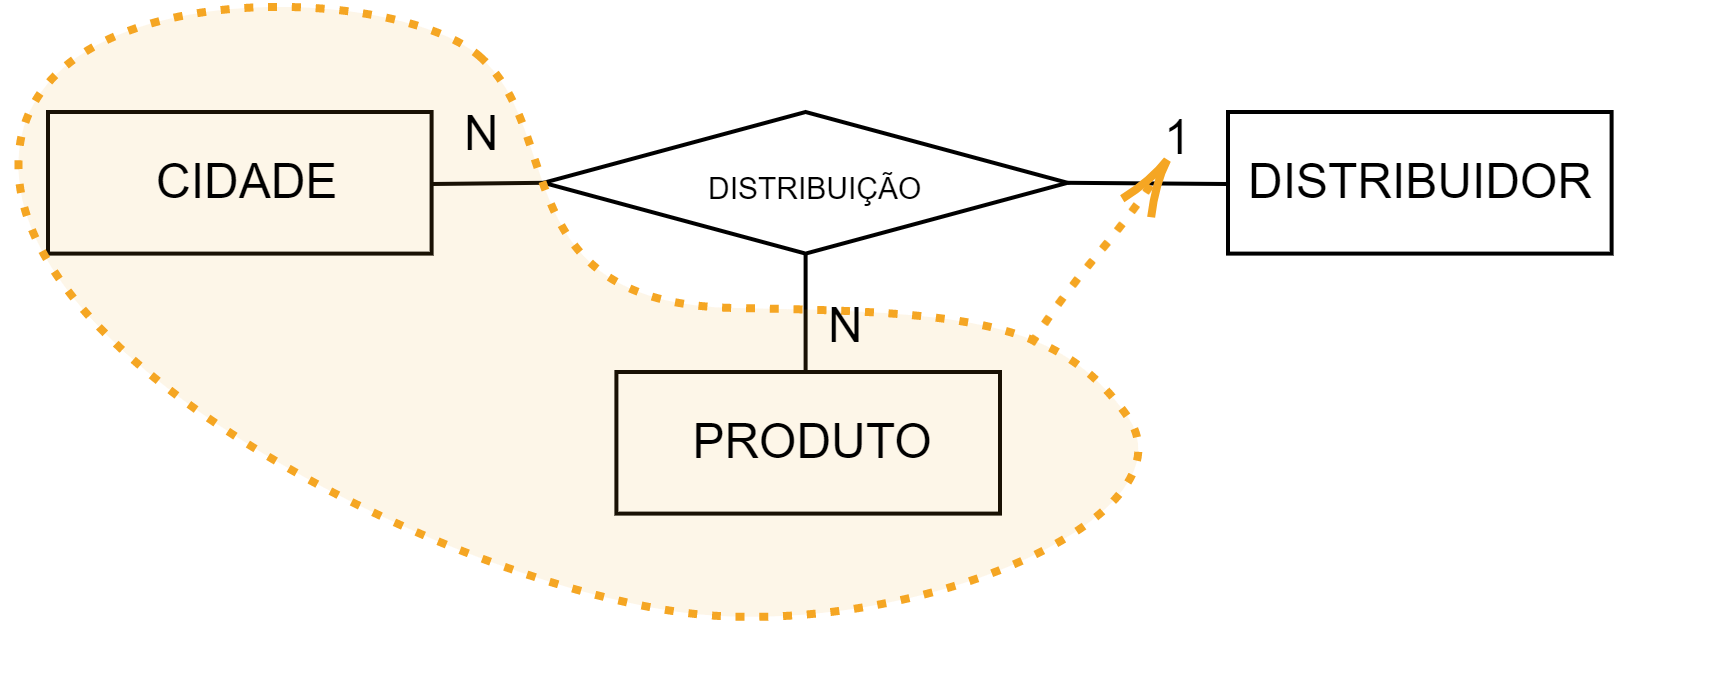
\includegraphics[scale=0.2]{Figuras/01_27.png}
\end{figure}

\end{ftst}

%==================================

\begin{ftst}{Restrições sobre relacionamentos ternários
(ou n-ários)}{Modelo Entidade-Relacionamento}

\begin{figure}
    \centering
    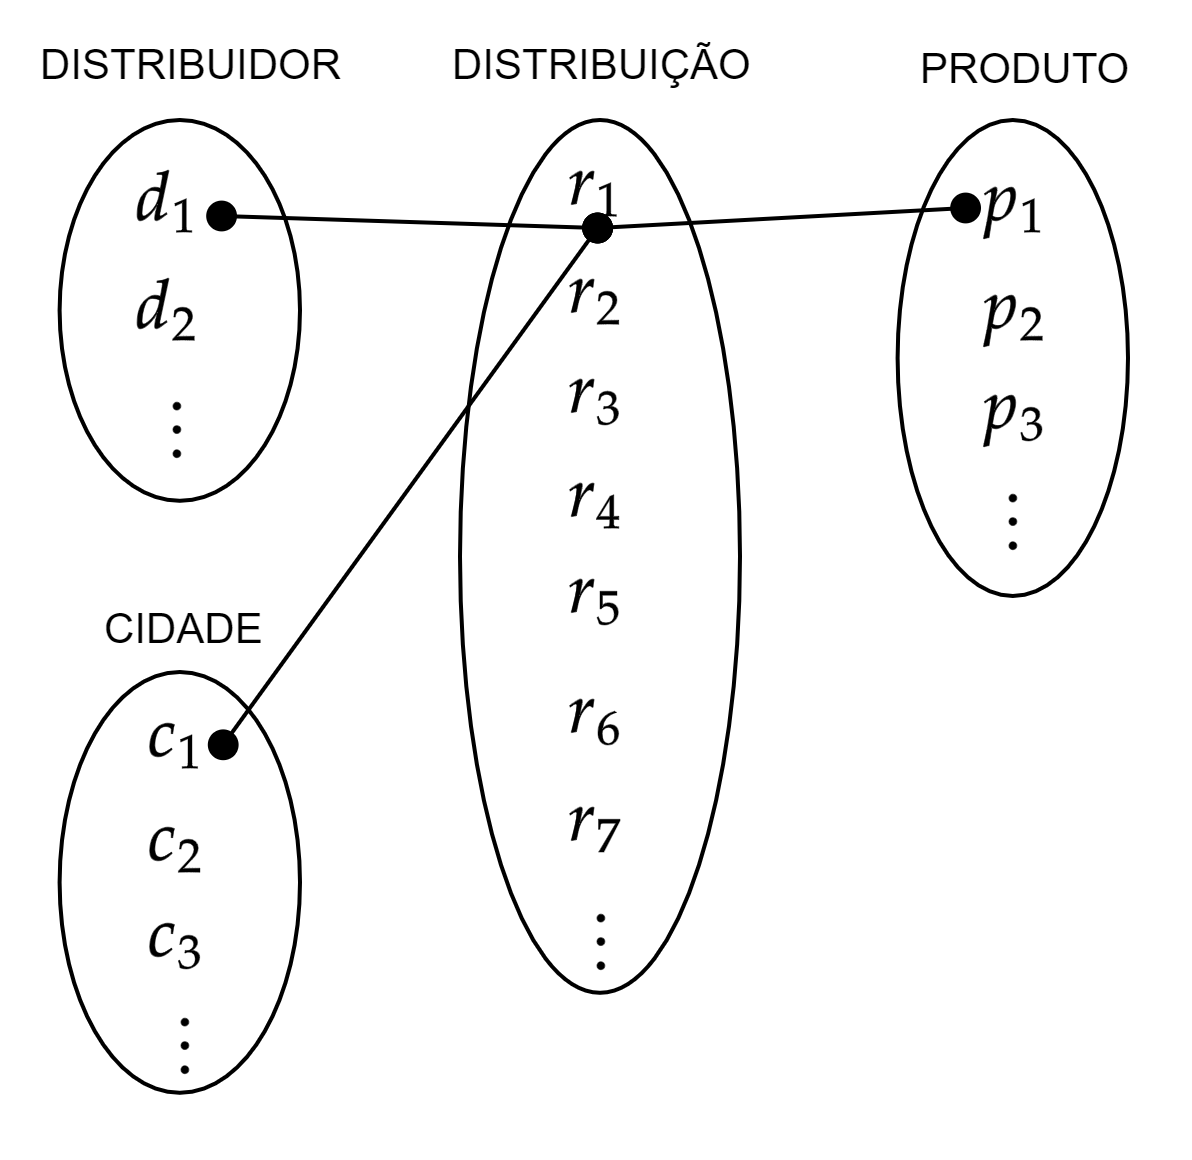
\includegraphics[scale=0.16]{Figuras/01_31.png}
\end{figure}

\end{ftst}

%==================================

\begin{ftst}{Restrições sobre relacionamentos ternários
(ou n-ários)}{Modelo Entidade-Relacionamento}

\begin{figure}
    \centering
    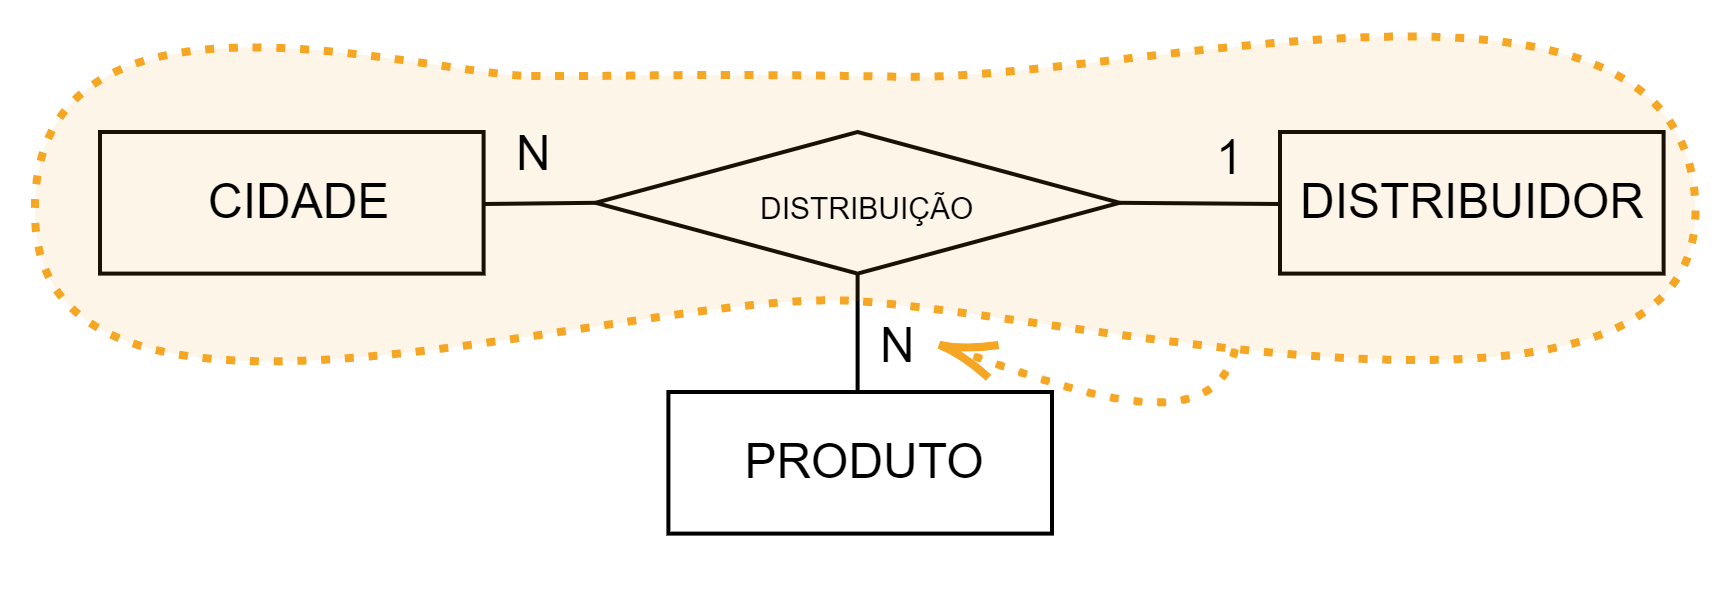
\includegraphics[scale=0.2]{Figuras/01_28.png}
\end{figure}

\end{ftst}

%==================================

\begin{ftst}{Restrições sobre relacionamentos ternários
(ou n-ários)}{Modelo Entidade-Relacionamento}

\begin{figure}
    \centering
    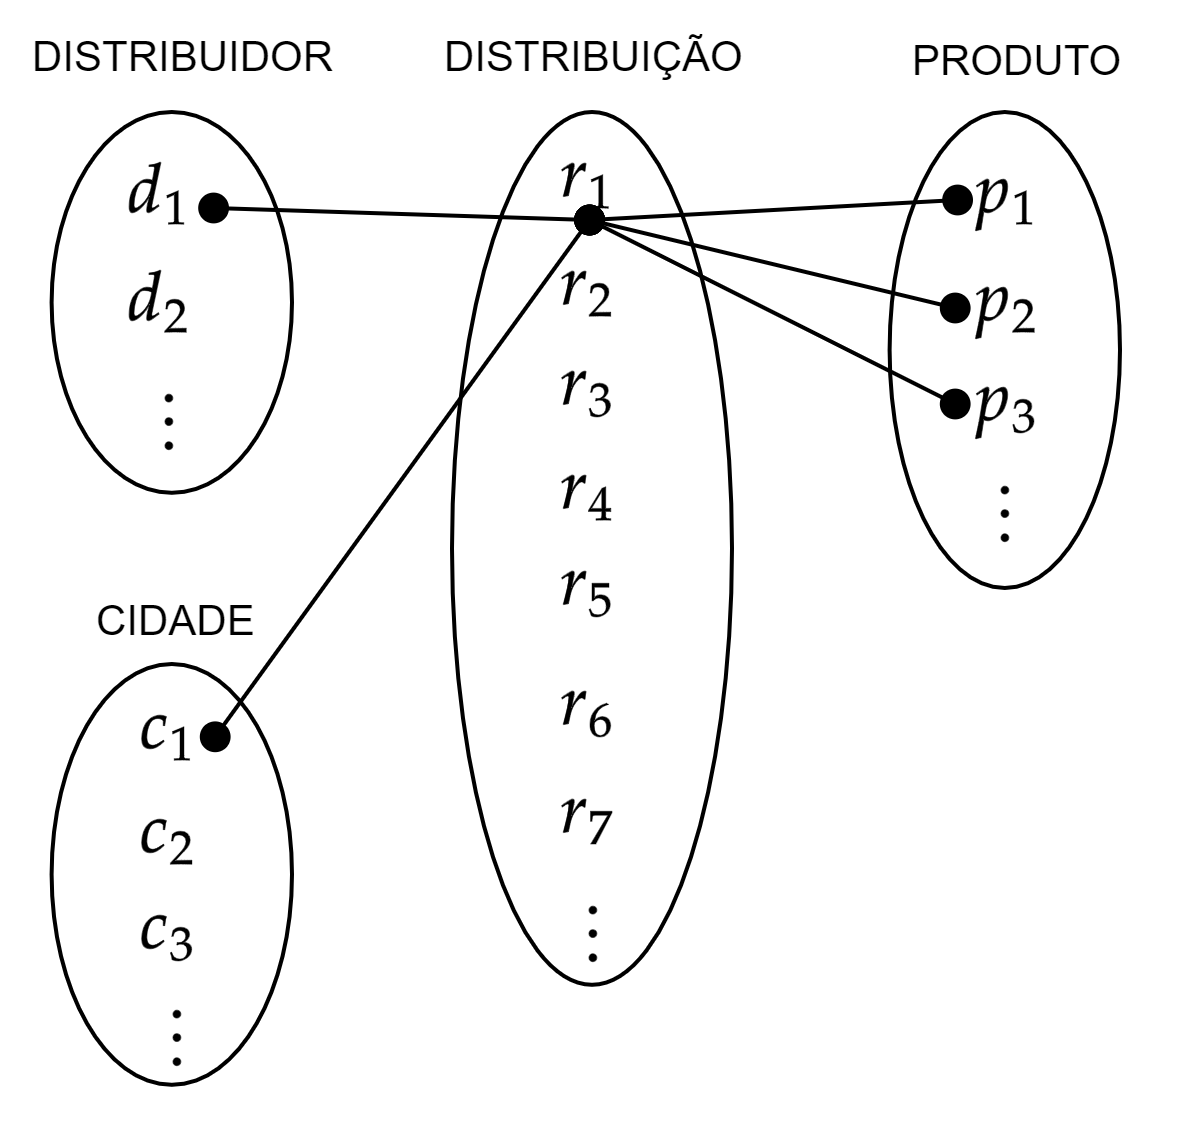
\includegraphics[scale=0.16]{Figuras/01_30.png}
\end{figure}

\end{ftst}

%==================================

\begin{ftst}{DER: nomeação apropriada}{Modelo Entidade-Relacionamento}
\small
\begin{itemize}
    \item Ao projetar um esquema de banco de dados, a escolha de nomes para entidades, atributos, relacionamentos e papéis nem sempre é simples.
    \item E preciso escolher nomes que transmitam, tanto quanto possível, os significados associados às diferentes construções no esquema. 
    \item Escolha nomes no singular para as entidades.
    \item Padronize o DER, use, por exemplo: entidades e relacionamentos são escritos com letras maiúsculas, os nomes dos atributos têm apenas a letra inicial maiúscula e os nomes do papel são escritos com letras minúsculas.
    \item Como uma prática geral, dada uma descrição narrativa dos requisitos do banco de dados, os substantivos que aparecem na narrativa tendem a gerar nomes de entidades, e os verbos tendem a indicar nomes de relacionamentos. 
\end{itemize}
\end{ftst}

%==================================

\begin{ftst}{Praticando 1}{Modelo Entidade-Relacionamento}

Nesse exercício vamos modelar os dados de uma livraria. Use os requisitos abaixo para criar um diagrama entidade-relacionamento completo e legível.
\vone
\begin{itemize}
    \item Precisamos manter informações dos livros disponíveis para a venda. Para cada livro deve ser armazenado seu ISBN, título, idioma e ano de lançamento, o(s) autor(es) e a editora.
    \item Para os autores é mantido o nome, data de nascimento, país de origem e uma breve nota biográfica.
    \ite Cada livro é escrito por um ou mais autores e para um mesmo autor podem existir vários livros cadastrados.
    \item Um autor pode estar incluído no cadastro mesmo que não exista um livro seu para venda.
    
\end{itemize}

\end{ftst}

%==================================

\begin{ftst}{Praticando 1}{Modelo Entidade-Relacionamento}


\begin{itemize}
    \item A livraria mantém também um cadastro de editoras que deve conter o nome, razão social, endereço (rua, número, bairro e cidade) e telefones de contato.
    \item Uma editora pode estar cadastrada mesmo quando não existam livros editados por ela em venda.
    \item Para um mesmo livro podem existir várias edições publicadas em anos distintos.
    \item Cada edição deverá ter um número, preço de venda, número de páginas e quantidade de exemplares em estoque.
\end{itemize}

\end{ftst}

%==================================

\begin{ftst}{Praticando 2}{Modelo Entidade-Relacionamento}
Nesse exercício vamos modelar os dados de uma universidade. Use os requisitos abaixo para criar um diagrama entidade-relacionamento completo e legível.
\vone
Deseja-se armazenar do aluno: quais disciplinas está matriculado, quais disciplinas já concluiu, qual seu curso, matrícula, nome, telefone, endereço (rua, número, bairro, cidade) e data de nascimento. Dos departamentos: código, nome e cursos que estão sob sua responsabilidade. Dos cursos: código, nome, disciplinas obrigatórias, disciplinas optativas, alunos matriculados e seu departamento. Das disciplinas: código, nome, alunos matriculados e pré-requisitos.

\end{ftst}

%==================================

\begin{ftst}{Praticando 3}{Modelo Entidade-Relacionamento}
Nesse exercício vamos modelar os dados de um sistema bancários. Use os requisitos abaixo para criar um diagrama entidade-relaciona- \\ mento completo e legível.
\vone
Para cada agência deseja-se armazenar seu número, cidade e seus funcionários. Dos funcionários devem ser armazenados: nome, endereço (rua, número, bairro e cidade), código, salário e telefones de contato. Cada cliente cadastrado em uma agência específica pode possuir várias contas bancárias.Para os clientes deseja-se armazenar o nome, o RG e a cidade na qual residem, além de suas contas bancárias. Dados importantes para as contas dos clientes da agência são o número da conta, o saldo e as informações sobre suas transações associadas a cada conta: número, data e valor.
\end{ftst}

%==================================

\begin{ftst}{Praticando 4}{Modelo Entidade-Relacionamento}
Nesse exercício vamos modelar os dados de uma agência de financiamento de projetos de pesquisa. Use os requisitos abaixo para criar um diagrama entidade-relacionamento completo e legível.
\vone
\small
\begin{itemize}
    \item Para cada projeto são cadastrados: um código interno, título, duração do projeto, instituição onde será realizado e área de pesquisa. As áreas de pesquisa estão predefinidas e para cada uma delas são cadastrados código, nome, descrição e um índice que indica sua relevância econômica. 
    \vone
    \item Para cada pesquisador solicitante são cadastrados RG, CPF, nome, sexo, data de nascimento, grau científico e instituição onde foi alcançado esse título. Note-se que um mesmo pesquisador pode ter vários projetos em análise. Um pesquisador é cadastrado no sistema unicamente quando o primeiro dos seus projetos é submetido.
\end{itemize}

\end{ftst}

\begin{ftst}{Praticando 4}{Modelo Entidade-Relacionamento}
\small
\begin{itemize}
    \item A agência recebe os projetos submetidos pelos pesquisadores e associa cada um destes a um avaliador que deve aprovar ou não o financiamento. Para estes avaliadores são cadastrados RG, CPF, nome, sexo, data de nascimento, grau científico, instituição onde trabalha e as áreas de pesquisa (anteriormente citadas) nas quais tem capacidade de avaliar os projetos.
    \vone
    \item Um avaliador pode ser cadastrado no sistema mesmo sem ter analisado nenhum projeto. Quando um projeto é enviado a um avaliador para análise, é cadastrada pelo sistema a data deste envio. Posteriormente, quando o avaliador retorna sua avaliação, são também cadastrados a data de resposta e o resultado (se foi aprovado ou não o projeto).
\end{itemize}
\end{ftst}


\end{document}
